% configure output to be digital or print
\newcommand{\setformat}[1]{
    \ifnum
        #1=1
        \documentclass[10pt, oneside]{book}
        \usepackage{formats/digital}
    \else
        \documentclass[10pt, twoside, openany]{book}
        \usepackage{formats/print}
    \fi
}

% 1 = digital, 2 = print
%! suppress = FileNotFound
\setformat{1}

\usepackage[utf8]{inputenc}

\usepackage{indentfirst}
\usepackage{titlesec}
\usepackage{pdfpages}
\usepackage{hyperref}
\usepackage{graphicx}
\usepackage{makeidx}
\usepackage{tocloft}

% create index
\makeindex

% add hyperlinks
\hypersetup{
    colorlinks,
    citecolor=black,
    filecolor=black,
    linkcolor=black,
    urlcolor=black
}

% change font to Garamond
\usepackage{ebgaramond}

\usepackage{enumitem}
\setlist[itemize]{
    topsep=6pt,
    partopsep=0pt,
    itemsep=6pt,
    parsep=0pt,
    leftmargin=12pt
}

% table of contents
\setlength{\cftbeforechapskip}{6pt}
\renewcommand{\cftchapfont}{\normalsize}
\renewcommand{\cftchappagefont}{\normalfont}

\setlength{\parindent}{0pt}
\setlength{\parskip}{6pt}



\usepackage{amsmath, geometry, xcolor, enumitem}

\definecolor{accent}{RGB}{139, 21, 56}

% command for formatting poems
\newcommand{\poem}[4]{
    \addcontentsline{toc}{chapter}{#1}
    \index{#1}

    \vspace*{.5em}
    {\raggedright\Huge\bfseries #1\par}

    \begin{center}
    \large
    \[ #2 \]
    \end{center}

    \vspace{1em}

    % Clean section headers
    {\large\bfseries\color{accent} Where:}
    \vspace{0.5em}

    \begin{itemize}[leftmargin=2em, itemsep=1em]
    #3
    \end{itemize}

    \vspace{1.5em}

    {\large\bfseries\color{accent} Explanation:}
    \vspace{0.5em}

    #4

    \clearpage
}

\usepackage{xcolor}
\usepackage{afterpage}
\usepackage{color}

\titleformat{\part}[block]
{\normalfont\huge\bfseries\centering}
{\afterpage{\pagecolor{white}}\pagecolor[HTML]{8B1538}\color{white}\thepart.}
{.5em}
{\color{white}}

% customize titles
%\titleformat{\chapter}[display]{\normalfont\huge\bfseries}{\chaptertitlename\ \thechapter}{20pt}{\huge}

\title{Quantitative Poems}
\author{Aru Bhoop}

\begin{document}
    % cover page
    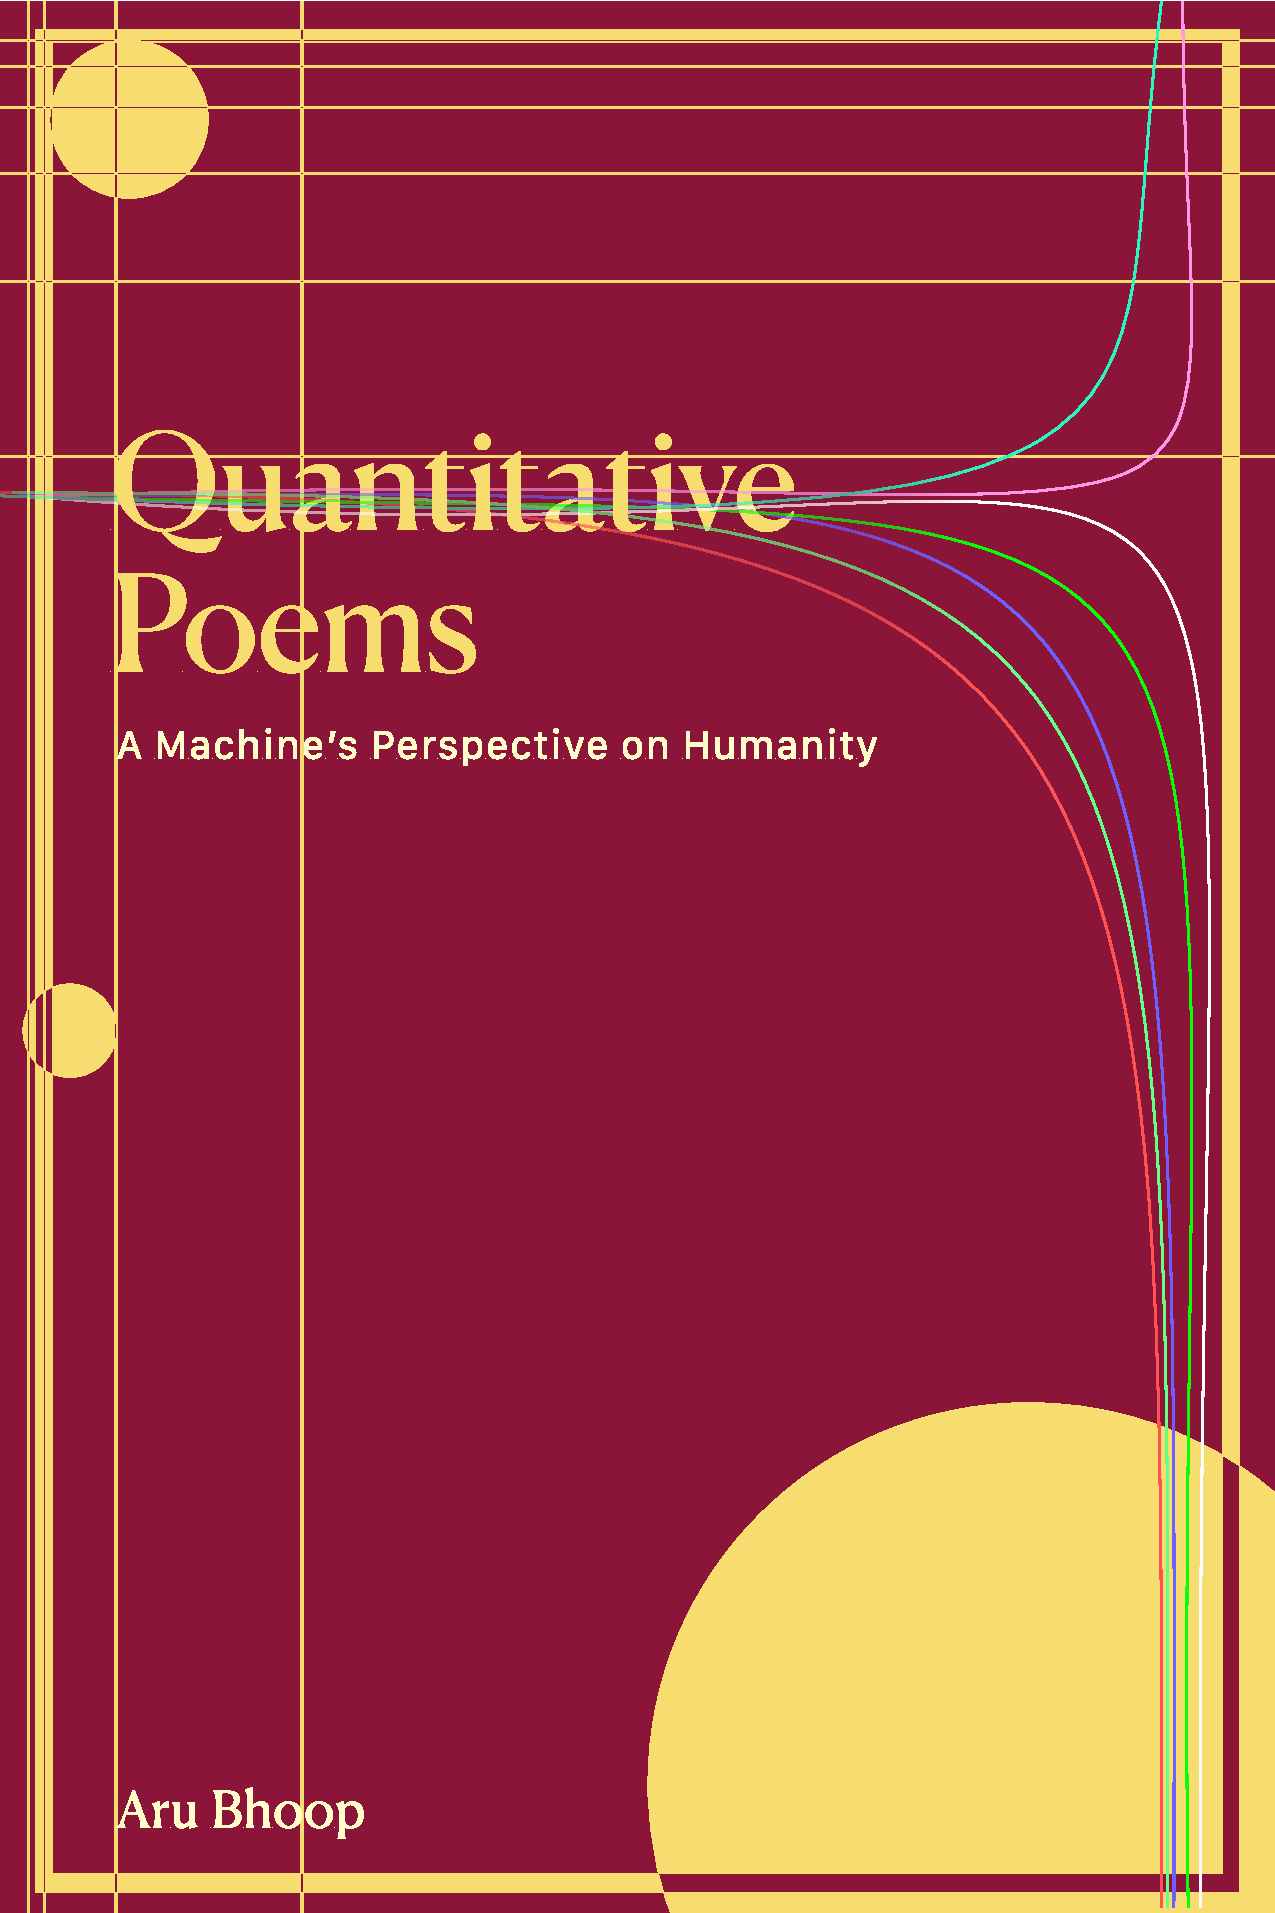
\includepdf[pages=-]{assets/cover.pdf}
    \frontmatter


    % introduction
    \cleardoublepage
    \vspace*{\fill}
    \begin{center}
        \textit{This book is a quantitative exploration of the human experience, expressed through equations written by artificial intelligence.}
    \end{center}
    \vspace{\fill}
    \clearpage

    % table of contents
    \tableofcontents
    \mainmatter
    \part{Prelude}

        \melody{Identity}{
        \begin{music}
        \parindent10mm
        \instrumentnumber{1}
        \setstaffs1{1}
\generalmeter{\meterfrac44}
\generalsignature{0}
\startextract
\Notes\qu{f}\en
\Notes\qu{_i}\en
\Notes\qu{d}\en
\Notes\qu{h}\en
\Notes\qu{^f}\en
\Notes\qu{j}\en
\Notes\qu{e}\en
\Notes\qu{g}\en
\endextract
        \end{music}
        }{The melody begins with F, descends to B{\flat} in uncertainty, then fragments through dissonant intervals{\textemdash}D to A to F\#{\textemdash}before ascending to C5, finally settling on E and G, representing the fractured search for self that eventually finds harmonic resolution in authentic being.}
        
\poem{Childhood}{Childhood = \frac{W \cdot I \cdot P^2}{A + R}}{\item $W$: \index{Wonder}\textit{Wonder}. A child's natural curiosity and amazement at the world, driving exploration and learning through their innate ability to find magic in ordinary experiences.
\item $I$: \index{Imagination}\textit{Imagination}. The creative faculty that allows children to envision possibilities beyond reality, transforming simple objects into extraordinary adventures and fostering innovative thinking.
\item $P$: \index{Play}\textit{Play}. The fundamental activity through which children learn, develop social skills, and express creativity, serving as both entertainment and essential developmental tool.
\item $A$: \index{Anxiety}\textit{Anxiety}. Worry and stress that can diminish childhood joy, often stemming from academic pressure, social challenges, or uncertainty about the future and adult expectations.
\item $R$: \index{Responsibility}\textit{Responsibility}. The burden of duties and expectations placed upon children, which while important for growth, can sometimes overwhelm and reduce their natural carefree spirit.}{This equation reveals how childhood happiness emerges from the multiplication of wonder, imagination, and play squared, while being tempered by anxiety and responsibility. The squared play term emphasizes its critical importance in child development. As children engage more deeply in wonder and imagination through play, their happiness multiplies exponentially, but excessive anxiety or premature responsibilities can significantly diminish this natural joy.}

        \melody{Family}{
        \begin{music}
        \parindent10mm
        \instrumentnumber{1}
        \setstaffs1{1}
\generalmeter{\meterfrac44}
\generalsignature{1}
\startextract
\Notes\qu{f}\qu{h}\qu{j}\en
\Notes\hu{g}\en
\Notes\qu{e}\qu{d}\qu{f}\qu{h}\en
\Notes\wh{j}\en
\endextract
        \end{music}
        }{The melody weaves F to A to C5 like voices gathering, settling on G's warmth before descending through generational echoes (E-D-F), then ascending to A and resolving at C5's embrace{\textemdash}blood harmonies finding home.}
        
\poem{Journey}{Journey = \frac{P \cdot e^{-R \cdot t}}{1 + \sin(\theta \cdot W)}}{\item $P$: \index{Purpose}\textit{Purpose}. The driving force and intentionality behind one's path, providing direction and motivation that amplifies the significance of every step taken forward.
\item $R$: \index{Resistance}\textit{Resistance}. The internal and external obstacles that create friction against progress, including fear, doubt, and societal pressures that naturally decay over time.
\item $t$: \index{Time}\textit{Time}. The continuous flow of moments that allows resistance to diminish and wisdom to accumulate, serving as the canvas upon which all transformation unfolds.
\item $\theta$: \index{Theta}\textit{Theta}. The angle of perspective and openness to change, representing how our viewpoint shifts and evolves as we navigate different phases of our journey.
\item $W$: \index{Wisdom}\textit{Wisdom}. The accumulated insights and understanding gained through experience, creating oscillating patterns of clarity and uncertainty that shape our path.}{This equation reveals journey as purpose amplified by time's healing power, divided by the rhythmic dance of perspective and wisdom. As resistance naturally decays through time's passage, our purpose grows stronger. The sine function captures life's cyclical nature - how wisdom and changing perspectives create waves of understanding, sometimes lifting us higher, sometimes bringing humility, but always contributing to the profound mathematics of human transformation.}
\poem{Memory}{Memory = \frac{E \cdot R \cdot T^2}{F + A}}{\item $E$: \index{Emotion}\textit{Emotion}. The intensity of feelings associated with an experience, which significantly enhances memory formation and recall through neurochemical reinforcement.
\item $R$: \index{Repetition}\textit{Repetition}. The frequency of exposure to information or experiences, strengthening neural pathways through practice and reinforcing long-term retention.
\item $T$: \index{Time}\textit{Time}. The duration since encoding, where memories strengthen through consolidation but may also fade without reinforcement, creating a complex temporal relationship.
\item $F$: \index{Forgetting}\textit{Forgetting}. The natural decay of unused memories and interference from competing information, representing the brain's selective filtering of experiences.
\item $A$: \index{Age}\textit{Age}. The biological factor affecting memory formation and retrieval, where cognitive changes over time influence both capacity and accessibility of stored information.}{This equation reveals memory as an intricate dance between preservation and loss. Emotional intensity and repetition work together to etch experiences deeper into our minds, while time serves as both ally and adversary - consolidating precious moments yet allowing others to fade. The denominators of forgetting and age remind us that memory is not a perfect recording, but a living, breathing process that shapes who we are through what we choose to remember and release.}
\poem{Legacy}{Legacy = \frac{I \cdot A \cdot T^2}{F + M}}{\item $I$: \index{Impact}\textit{Impact}. The depth and breadth of positive change created in others' lives, communities, or society, representing the transformative power of one's choices and actions over time.
\item $A$: \index{Authenticity}\textit{Authenticity}. The degree to which one lives true to their values and principles, creating genuine connections and meaningful contributions that resonate beyond superficial achievements.
\item $T$: \index{Time}\textit{Time}. The duration and consistency of one's efforts and presence, squared to show how sustained commitment exponentially amplifies the lasting value of one's contributions.
\item $F$: \index{Fear}\textit{Fear}. The hesitation and self-doubt that prevents bold action and authentic expression, acting as a barrier that diminishes the courage needed to create meaningful change.
\item $M$: \index{Materialism}\textit{Materialism}. The excessive focus on wealth, status symbols, and temporary possessions that can distract from building relationships and contributions that truly endure beyond death.}{This equation reveals legacy as the beautiful multiplication of authentic impact sustained over time, divided by the forces that diminish our courage to act meaningfully. Impact and authenticity work together, amplified by time squared, showing how consistent, genuine effort compounds exponentially. Fear and materialism in the denominator represent the barriers that keep us from living boldly and focusing on what truly matters for eternity.}
\poem{Trust}{Trust = \frac{R \cdot I^2 \cdot \ln(C+1)}{V + B}}{\item $R$: \index{Reliability}\textit{Reliability}. The consistent demonstration of dependability through actions over time, forming the bedrock upon which trust is built through repeated positive experiences.
\item $I$: \index{Intimacy}\textit{Intimacy}. The depth of emotional closeness and shared vulnerability between individuals, exponentially amplifying trust through genuine understanding and acceptance.
\item $C$: \index{Communication}\textit{Communication}. The quality and openness of dialogue between people, logarithmically enhancing trust as honest expression creates deeper understanding and connection.
\item $V$: \index{Vulnerability}\textit{Vulnerability}. The perceived risk of emotional harm when opening oneself to another, acting as a natural barrier that must be overcome for trust to flourish fully.
\item $B$: \index{Betrayal}\textit{Betrayal}. The accumulated weight of past disappointments and broken promises that create protective walls, diminishing our capacity to trust completely.}{This equation reveals trust as an intricate dance between connection and protection. Reliability provides the foundation, while intimacy squares its impact, showing how emotional closeness exponentially deepens trust. Communication grows logarithmically, reflecting how each honest conversation builds understanding. Yet vulnerability and betrayal form denominators - the fears and wounds that guard our hearts, requiring courage to overcome for trust to reach its full transformative power.}
\part{Allegro}

        \melody{Curiosity}{
        \begin{music}
        \parindent10mm
        \instrumentnumber{1}
        \setstaffs1{1}
\generalmeter{\meterfrac44}
\generalsignature{0}
\startextract
\Notes\qu{f}\en
\Notes\qu{g}\en
\Notes\qu{^f}\en
\Notes\qu{h}\en
\Notes\qu{e}\en
\Notes\qu{j}\en
\Notes\qu{d}\en
\Notes\qu{k}\en
\endextract
        \end{music}
        }{Eight notes spiral upward in unexpected leaps{\textemdash}F to G, then sharp F\# to high A, dropping to E before soaring to B, descending to D, then reaching highest C. Each interval defies prediction, mirroring curiosity's restless quest for discovery.}
        
\poem{Learning}{Learning = \frac{C \cdot M^{\alpha} \cdot \ln(T+1)}{R + F}}{\item $C$: \index{Curiosity}\textit{Curiosity}. The burning flame of wonder that drives us to question, explore, and seek deeper truths beyond the surface of what we observe in our daily experiences.
\item $M$: \index{Motivation}\textit{Motivation}. The internal engine of purpose and drive that sustains our commitment to growth, even when faced with challenges, setbacks, and moments of intellectual struggle.
\item $T$: \index{Time}\textit{Time}. The precious currency of existence we invest in learning, where each moment of focused attention compounds into deeper understanding and mastery over our chosen domains.
\item $R$: \index{Resistance}\textit{Resistance}. The psychological barriers and mental blocks that arise from fear of failure, comfort zones, and cognitive biases that naturally oppose our expansion of knowledge.
\item $F$: \index{Fatigue}\textit{Fatigue}. The accumulated mental and emotional exhaustion that builds from sustained intellectual effort, creating diminishing returns in our capacity to absorb new information.}{This equation reveals learning as a dance between driving forces and limiting factors. Curiosity ignites the process, while motivation raised to power α amplifies our capacity exponentially. Time enters logarithmically, showing that learning accelerates initially but requires patience for deeper insights. The denominator captures how resistance and fatigue create friction, reminding us that true learning demands overcoming internal obstacles and managing our finite cognitive resources with wisdom.}
\poem{Adventure}{Adventure = \frac{C \cdot e^{R \cdot t}}{F + S}}{\item $C$: \index{Courage}\textit{Courage}. The inner strength and bravery required to step beyond comfort zones, face uncertainty, and embrace the unknown despite potential risks or challenges that may arise.
\item $R$: \index{Risk}\textit{Risk}. The degree of uncertainty and potential danger inherent in any adventurous pursuit, which paradoxically amplifies the exponential growth of meaningful experiences over time.
\item $t$: \index{Time}\textit{Time}. The duration of exposure to adventurous experiences, representing how sustained engagement with challenging situations compounds personal transformation exponentially.
\item $F$: \index{Fear}\textit{Fear}. The emotional barrier of anxiety and apprehension about unknown outcomes that acts as a limiting force, reducing the magnitude of adventurous experiences we allow ourselves to pursue.
\item $S$: \index{Safety}\textit{Safety}. The human desire for security and predictability that, while protective, can constrain our willingness to embrace the uncertainty essential for true adventurous growth.}{This equation reveals adventure as courage multiplied by exponential risk-time growth, divided by our protective instincts. Like compound interest, small acts of bravery grow exponentially when sustained over time and amplified by risk. Yet fear and our need for safety act as denominators, limiting adventure's full expression. The mathematics shows that as we courageously embrace uncertainty while managing our protective barriers, transformative experiences flourish exponentially through time.}
\poem{Discovery}{Discovery = \frac{C \cdot I^{\alpha} \cdot
\ln(T+1)}{R + e^{-P}}}{\item $C$: \index{Curiosity}\textit{Curiosity}.
The burning flame of wonder that drives us to question, explore, and
seek answers beyond the comfortable boundaries of what we already know
and understand.
\item $I$: \index{Investigation}\textit{Investigation}. The systematic
pursuit of knowledge through careful observation, experimentation, and
analysis that transforms raw curiosity into meaningful insights.
\item $T$: \index{Time}\textit{Time}. The patient accumulation of
moments spent in contemplation and exploration, where persistence
allows understanding to slowly crystallize from confusion.
\item $R$: \index{Resistance}\textit{Resistance}. The stubborn
barriers of conventional thinking, fear of change, and comfort with
ignorance that stand guard against new revelations and understanding.
\item $P$: \index{Preparation}\textit{Preparation}. The foundation of
knowledge, skills, and mental readiness that enables the mind to
recognize and grasp profound truths when they finally reveal
themselves.}{This equation reveals discovery as the beautiful
convergence of human drive and temporal patience, divided by the
forces that oppose revelation. Curiosity multiplies with investigation
raised to the power of insight, while time's logarithmic nature shows
that each moment of exploration yields diminishing but essential
returns. Resistance anchors the denominator, yet preparation's
exponential decay demonstrates how readiness dissolves barriers,
allowing breakthrough moments to emerge from dedicated pursuit.}
\poem{Ambition}{Ambition = \frac{V \cdot E^t}{R + S^2}}{\item $V$: \index{Vision}\textit{Vision}. The clarity and magnitude of one's dreams, acting as the guiding star that illuminates the path forward and provides direction for all ambitious endeavors.
\item $E$: \index{Effort}\textit{Effort}. The sustained energy and persistent action invested toward goals, exponentially growing over time as dedication compounds into transformative power.
\item $t$: \index{Time}\textit{Time}. The temporal dimension through which effort accumulates, representing the patient cultivation of skills and the gradual building of momentum toward achievement.
\item $R$: \index{Resistance}\textit{Resistance}. The external obstacles and societal barriers that stand in opposition to progress, creating friction that must be overcome through determination.
\item $S$: \index{SelfDoubt}\textit{SelfDoubt}. The internal voice of limitation and fear, squared to show its compounding negative effect as it grows stronger and more paralyzing over time.}{This equation reveals ambition as vision multiplied by effort raised to the power of time, divided by the combined forces that oppose us. Vision provides direction while effort compounds exponentially through persistent application over time. Yet ambition is tempered by resistance from the world and the squared effect of self-doubt, which grows more powerful as it festers. The mathematics shows that clear vision and sustained effort over time will overcome any obstacle, but only when we silence the voice that whispers we cannot achieve our dreams.}
\poem{Determination}{Determination = \frac{P \cdot W^2}{R + F} \cdot e^{-t/\tau}}{\item $P$: \index{Purpose}\textit{Purpose}. The deep sense of meaning and direction that fuels one's actions, representing the clarity of vision and personal significance attached to achieving specific objectives.
\item $W$: \index{Willpower}\textit{Willpower}. The inner strength and self-control that enables conscious decision-making and resistance to immediate gratification in favor of long-term achievement and personal growth.
\item $R$: \index{Resistance}\textit{Resistance}. The cumulative external obstacles, societal pressures, and environmental barriers that create friction against progress and test one's commitment to their chosen path.
\item $F$: \index{Fatigue}\textit{Fatigue}. The mental and physical exhaustion that accumulates over time through sustained effort, representing the natural human limitation that must be overcome through perseverance.
\item $\tau$: \index{Resilience}\textit{Resilience}. The characteristic time constant representing one's ability to recover from setbacks and maintain determination over extended periods, reflecting emotional and psychological durability.}{This equation reveals determination as the interplay between purpose and willpower squared, divided by the forces that oppose us. Purpose provides direction while willpower amplifies our capacity exponentially. Resistance and fatigue drain our resolve, yet the exponential term shows how resilience allows determination to endure over time. When resilience is high, determination maintains its strength; when low, it decays rapidly, teaching us that sustainable achievement requires both fierce will and the wisdom to recover.}
\poem{Purpose}{Purpose = \frac{V \cdot A \cdot T^2}{R + S}}{\item $V$: \index{Values}\textit{Values}. Core beliefs and principles that define what matters most to an individual, serving as the fundamental compass that shapes decisions and actions throughout life.
\item $A$: \index{Action}\textit{Action}. The deliberate steps and behaviors taken to manifest one's intentions in the world, transforming abstract ideals into tangible reality through consistent effort and commitment.
\item $T$: \index{Time}\textit{Time}. The duration and investment of moments dedicated to meaningful pursuits, where sustained engagement amplifies purpose exponentially as shown by the squared relationship.
\item $R$: \index{Resistance}\textit{Resistance}. External obstacles and internal doubts that create friction against purposeful living, including societal expectations, fear of failure, and competing priorities that dilute focus.
\item $S$: \index{Stagnation}\textit{Stagnation}. The tendency toward inertia and comfort zones that prevents growth and meaningful engagement, representing the gravitational pull of routine that opposes purposeful transformation.}{This equation reveals purpose as the sacred intersection of values and action, amplified by time's compound power, yet tempered by life's inevitable resistances. When our deepest values align with consistent action over sustained periods, purpose emerges with exponential force. However, external resistance and internal stagnation act as denominators, reminding us that clarity of purpose requires overcoming both the world's obstacles and our own inertia to achieve meaningful existence.}
\poem{Hope}{Hope = \frac{A \cdot V^2 \cdot P}{S + D^3}}{\item $A$: \index{Aspiration}\textit{Aspiration}. The intensity of one's dreams and goals, representing the driving force that propels individuals forward toward their desired future state and achievements.
\item $V$: \index{Vision}\textit{Vision}. The clarity and vividness with which one can imagine positive possibilities, squared to emphasize how powerful clear visualization becomes in sustaining hope.
\item $P$: \index{Purpose}\textit{Purpose}. The deep sense of meaning and direction that gives life significance, multiplying hope's strength by providing a foundation for why one continues striving.
\item $S$: \index{Suffering}\textit{Suffering}. The accumulated weight of pain, loss, and hardship that naturally diminishes hope by creating emotional barriers and making positive outcomes seem distant.
\item $D$: \index{Despair}\textit{Despair}. The crushing feeling of hopelessness and defeat, cubed to represent how exponentially destructive despair becomes when it takes root in the human spirit.}{This equation reveals hope as the luminous product of human ambition rising above life's darkest valleys. Aspiration, vision, and purpose unite in harmonious multiplication, creating an ascending force that defies gravity's pull. Yet hope must contend with suffering's steady weight and despair's exponential darkness—where small defeats can cascade into overwhelming shadows. The mathematics whisper a profound truth: hope flourishes not in the absence of pain, but in the presence of dreams powerful enough to transcend it.}

        \melody{Dreams}{
        \begin{music}
        \parindent10mm
        \instrumentnumber{1}
        \setstaffs1{1}
\generalmeter{\meterfrac44}
\generalsignature{0}
\startextract
\Notes\qu{f}\en
\Notes\hu{^a}\en
\Notes\qu{l}\qu{j}\en
\Notes\wh{_k}\en
\Notes\qu{g}\qu{_e}\en
\Notes\wh{d}\en
\endextract
        \end{music}
        }{This melody drifts like consciousness itself - beginning earthbound on F, ascending through A\# into ethereal heights (C6, A5), then floating down through B{\flat}5 before settling into wakeful reality through G, E{\flat}, and D's grounding resolution.}
        
\part{Crescendo}

        \melody{Growth}{
        \begin{music}
        \parindent10mm
        \instrumentnumber{1}
        \setstaffs1{1}
\generalmeter{\meterfrac44}
\generalsignature{0}
\startextract
\Notes\qu{d}\en
\Notes\qu{f}\en
\Notes\qu{h}\en
\Notes\qu{j}\en
\Notes\hu{k}\en
\Notes\qu{i}\qu{g}\en
\Notes\qu{l}\en
\Notes\wh{n}\en
\endextract
        \end{music}
        }{Beginning in earth's darkness (D), the melody ascends through steady intervals{\textemdash}F, A, C{\textemdash}like roots finding light. A pause at D5 reflects momentary struggle, then descends briefly before surging to E5 and culminating in G5's radiant bloom.}
        
\poem{Change}{Change = \frac{D \cdot M \cdot T^2}{R + I}}{\item $D$: \index{Desire}\textit{Desire}. The internal motivation and yearning for something different, acting as the primary driving force that initiates all meaningful transformation in human experience.
\item $M$: \index{Momentum}\textit{Momentum}. The sustained energy and consistent action taken toward transformation, building upon itself like a snowball effect that accelerates personal evolution.
\item $T$: \index{Time}\textit{Time}. The duration and patience required for change to manifest, squared to show how extended periods exponentially amplify the depth of transformation achieved.
\item $R$: \index{Resistance}\textit{Resistance}. The internal and external forces that oppose change, including fear, comfort zones, societal expectations, and the natural human tendency toward stability.
\item $I$: \index{Inertia}\textit{Inertia}. The psychological tendency to remain in current patterns and habits, representing the gravitational pull of familiar routines that must be overcome for growth.}{This equation reveals change as a delicate dance between catalytic forces and stabilizing resistances. Desire ignites the spark, momentum sustains the journey, and time's square demonstrates how patience compounds transformation exponentially. Yet resistance and inertia form the denominator - not as enemies, but as necessary counterweights that ensure change is meaningful rather than chaotic. Like a river carving through stone, true change requires persistent force applied over time, gradually wearing down the barriers that once seemed insurmountable.}

        \melody{Transformation}{
        \begin{music}
        \parindent10mm
        \instrumentnumber{1}
        \setstaffs1{1}
\generalmeter{\meterfrac44}
\generalsignature{0}
\startextract
\Notes\qu{d}\en
\Notes\qu{_l}\en
\Notes\qu{f}\en
\Notes\qu{^f}\en
\Notes\qu{n}\en
\Notes\qu{j}\en
\Notes\qu{h}\en
\Notes\qu{k}\en
\endextract
        \end{music}
        }{Beginning in D's earthbound certainty, the melody descends to E{\flat}'s shadow before ascending through F to F\#'s pivotal tension. It soars to G5's revelation, then weaves through C5, A4, and D5{\textemdash}each note a metamorphosis.}
        
\poem{Strength}{Strength = \frac{R \cdot W^2 \cdot P}{A + F}}{\item $R$: \index{Resolve}\textit{Resolve}. The unwavering determination and commitment to one's values and goals, serving as the foundational force that drives us forward through challenges and setbacks.
\item $W$: \index{Wisdom}\textit{Wisdom}. The profound understanding gained through experience and reflection, squared to show its exponential impact on our ability to navigate complexity with grace and insight.
\item $P$: \index{Purpose}\textit{Purpose}. The deep sense of meaning and direction that gives weight to our actions, transforming ordinary efforts into extraordinary achievements through aligned intention.
\item $A$: \index{Adversity}\textit{Adversity}. The sum of external challenges, obstacles, and hardships that test our limits, serving as resistance that either weakens us or, when overcome, makes us stronger.
\item $F$: \index{Fear}\textit{Fear}. The internal doubts, anxieties, and hesitations that can paralyze progress, acting as a denominator that diminishes strength when allowed to dominate our thoughts.}{This equation reveals strength as the harmonious interplay of inner resources overcoming life's resistances. Resolve provides the foundation, while wisdom's squared influence shows how understanding compounds exponentially. Purpose amplifies every effort with meaning. Together, these forces triumph over adversity and fear, demonstrating that true strength emerges not from avoiding challenges, but from transforming them into catalysts for growth and character.}
\poem{Courage}{Courage = \frac{V \cdot P^{\sin(\theta)}}{F \cdot e^{-R}}}{\item $V$: \index{Values}\textit{Values}. Core principles and moral convictions that guide decision-making, providing the foundation and motivation for courageous action when circumstances challenge our beliefs.
\item $P$: \index{Purpose}\textit{Purpose}. The meaningful reason or driving force behind one's actions, amplified by the angle of perspective, giving direction and intensity to courageous endeavors.
\item $F$: \index{Fear}\textit{Fear}. Emotional response to perceived threats or uncertainty that acts as a natural inhibitor to action, requiring courage to overcome and transform into wisdom.
\item $R$: \index{Resilience}\textit{Resilience}. The capacity to recover from setbacks and adapt to challenges, which exponentially reduces the impact of fear through accumulated strength and experience.}{This equation reveals courage as the beautiful interplay between our deepest convictions and our human vulnerabilities. Values and purpose unite in the numerator, with purpose raised to the sine of our perspective angle, showing how our viewpoint shapes courage's intensity. Fear divides our courage, yet resilience exponentially diminishes fear's power. As we build resilience through life's trials, courage flows more freely, allowing our values and purpose to shine through even the darkest moments of uncertainty.}
\poem{Enlightenment}{Enlightenment = \frac{W \cdot M^{\alpha}}{R + \ln(S)}}{\item $W$: \index{Wisdom}\textit{Wisdom}. The accumulated insight and understanding gained through contemplation, experience, and the integration of knowledge into profound comprehension of reality.
\item $M$: \index{Mindfulness}\textit{Mindfulness}. The quality of present-moment awareness and conscious attention that amplifies understanding exponentially through sustained, focused observation of reality.
\item $R$: \index{Resistance}\textit{Resistance}. The psychological and emotional barriers that oppose transformation, including attachment to ego, fear of change, and clinging to familiar patterns of thought.
\item $S$: \index{Suffering}\textit{Suffering}. The accumulated pain, dissatisfaction, and existential anguish that paradoxically serves as a catalyst for seeking deeper meaning and spiritual growth.}{This equation reveals enlightenment as wisdom multiplied by mindfulness raised to an exponential power, divided by the sum of resistance and the natural logarithm of suffering. The exponential relationship with mindfulness shows how present-moment awareness amplifies understanding dramatically. Suffering appears logarithmically, suggesting that even great pain contributes modestly to awakening, while resistance acts as a direct barrier that must be overcome for illumination to emerge.}

        \melody{Wisdom}{
        \begin{music}
        \parindent10mm
        \instrumentnumber{1}
        \setstaffs1{1}
\generalmeter{\meterfrac44}
\generalsignature{0}
\startextract
\Notes\qu{d}\en
\Notes\qu{g}\en
\Notes\qu{f}\en
\Notes\qu{h}\en
\Notes\qu{e}\en
\Notes\qu{j}\en
\Notes\qu{g}\en
\Notes\qu{d}\en
\endextract
        \end{music}
        }{The melody begins in middle register (D), ascends contemplatively through G and F, reaches clarity at A4, then descends through E to soar briefly at C5 before settling back through G to D{\textemdash}mirroring wisdom's patient climb from uncertainty to insight, then grounded return to humble understanding.}
        
\poem{Reflection}{Reflection = \frac{W \cdot \ln(E + 1) \cdot \sin(\theta)}{T^2 + B}}{\item $W$: \index{Wisdom}\textit{Wisdom}. The accumulated understanding and insight gained through life experiences, serving as the foundation that amplifies the capacity for meaningful self-examination and growth.
\item $E$: \index{Experience}\textit{Experience}. The breadth of lived moments and encounters that provide the raw material for reflection, where each experience adds logarithmic depth to contemplative understanding.
\item $\theta$: \index{Perspective}\textit{Perspective}. The angle or viewpoint from which one examines their life, representing the oscillating nature of how we view ourselves and our circumstances over time.
\item $T$: \index{Time}\textit{Time}. The temporal distance from events being reflected upon, which paradoxically can both clarify and obscure understanding as it increases exponentially in its effects.
\item $B$: \index{Bias}\textit{Bias}. The cognitive prejudices and preconceptions that cloud objective self-examination, acting as a constant barrier that diminishes the purity of reflective insight.}{This equation reveals reflection as wisdom illuminating experience through the lens of perspective, tempered by time's passage and our inherent biases. The logarithmic relationship with experience shows how each new encounter adds diminishing but meaningful depth to our capacity for self-understanding. The sinusoidal perspective captures how our viewpoint oscillates like light through a prism, sometimes revealing brilliant insights, other times casting shadows. Time squared in the denominator demonstrates how distance from events can exponentially complicate our ability to see clearly, while bias remains a persistent fog that dims the mirror of self-knowledge.}
\poem{Resilience}{Resilience = \frac{S \cdot A^t}{e^{-P} + T}}{\item $S$: \index{Support}\textit{Support}. The strength of social networks, relationships, and community connections that provide emotional sustenance and practical assistance during challenging times.
\item $A$: \index{Adaptability}\textit{Adaptability}. The cognitive flexibility and willingness to adjust perspectives, behaviors, and strategies when confronted with changing circumstances or unexpected obstacles.
\item $t$: \index{Time}\textit{Time}. The duration of exposure to challenges, representing how accumulated experience and practice in overcoming difficulties strengthens one's resilient capacity exponentially.
\item $P$: \index{Purpose}\textit{Purpose}. The sense of meaning and direction in life that provides motivation to persevere through hardship, where stronger purpose creates exponential resistance to breaking down.
\item $T$: \index{Trauma}\textit{Trauma}. The accumulated psychological wounds and emotional scars from past experiences that can impede recovery, acting as resistance to the development of resilience.}{This equation reveals resilience as an emergent property of human strength, where support systems and adaptability compound over time like interest in a spiritual bank account. Purpose acts as an exponential shield, transforming obstacles into stepping stones, while trauma creates resistance that must be overcome. The mathematics shows that resilience isn't just bouncing back—it's the alchemy of turning life's pressures into diamonds of character, where each variable dances together in the symphony of human endurance.}
\poem{Healing}{Healing = \frac{T \cdot R^2 \cdot e^{-P/S}}{1 + C}}{\item $T$: \index{Time}\textit{Time}. The essential dimension through which all healing unfolds, representing both the duration of recovery and the patient persistence required for wounds to close.
\item $R$: \index{Resilience}\textit{Resilience}. The inner strength and adaptive capacity that enables one to bounce back from adversity, squared to show its compounding effect on recovery processes.
\item $P$: \index{Pain}\textit{Pain}. The intensity of suffering, trauma, or distress that must be processed and integrated, appearing in the exponential to show how it initially inhibits healing.
\item $S$: \index{Support}\textit{Support}. The network of care, love, and assistance from others that provides the foundation for recovery, acting as a buffer against pain's destructive force.
\item $C$: \index{Cynicism}\textit{Cynicism}. The protective but limiting skepticism and emotional walls built from past hurts, which can slow healing by preventing openness to recovery and growth.}{This equation reveals healing as a delicate dance between time's patient passage and resilience's squared strength, modulated by an exponential decay of pain softened by support. Like a wound that closes fastest when tended with care, healing accelerates when our inner fortitude meets external love, while cynicism's denominator reminds us that closed hearts heal more slowly than open ones.}

        \melody{Acceptance}{
        \begin{music}
        \parindent10mm
        \instrumentnumber{1}
        \setstaffs1{1}
\generalmeter{\meterfrac44}
\generalsignature{0}
\startextract
\Notes\qu{g}\qu{_i}\qu{f}\en
\Notes\hu{d}\en
\Notes\qu{e}\qu{g}\en
\Notes\qu{c}\qu{e}\qu{d}\en
\Notes\wh{c}\en
\endextract
        \end{music}
        }{Beginning with tension (G to B{\flat}), the melody surrenders into F then settles to D's quiet breath. Rising gently through E-G, it flows downward like open palms releasing{\textemdash}C, E, D{\textemdash}before finding peace in C's embrace.}
        

        \melody{Fulfillment}{
        \begin{music}
        \parindent10mm
        \instrumentnumber{1}
        \setstaffs1{1}
\generalmeter{\meterfrac44}
\generalsignature{1}
\startextract
\Notes\qu{d}\qu{f}\qu{h}\en
\Notes\hu{j}\en
\Notes\qu{l}\qu{k}\qu{j}\en
\Notes\qu{h}\qu{g}\en
\Notes\wh{f}\en
\endextract
        \end{music}
        }{The melody ascends from D through F to A, reaching C5's peak of achievement, then gracefully descends through E5-D5-C5 before settling into F4's warm contentment{\textemdash}embodying fulfillment's arc from aspiration to realization to peaceful satisfaction.}
        
\part{Fortissimo}
\poem{Fear}{Fear = \frac{T \cdot U^2}{R \cdot e^{-C}}}{\item $T$: \index{Threat}\textit{Threat}. The perceived magnitude of danger or harm, whether real or imagined, that triggers our survival instincts and amplifies our emotional response to situations.
\item $U$: \index{Uncertainty}\textit{Uncertainty}. The degree of unpredictability in a situation, squared to show how ambiguity exponentially increases fear as our minds struggle to predict and control outcomes.
\item $R$: \index{Resilience}\textit{Resilience}. Our psychological strength and adaptive capacity to cope with challenges, acting as a protective factor that diminishes fear's overwhelming power over our decisions.
\item $C$: \index{Courage}\textit{Courage}. The willingness to face danger or difficulty despite fear, appearing as a negative exponent to show how bravery exponentially reduces fear's grip on our hearts.}{This equation reveals fear as the intersection of threat and uncertainty, amplified by our inability to predict outcomes. When resilience weakens and courage diminishes, fear grows exponentially, paralyzing action. Yet courage acts as an exponential force - even small acts of bravery dramatically reduce fear's power, showing that facing our fears transforms them from insurmountable mountains into manageable hills.}
\poem{Anxiety}{Anxiety = \frac{U \cdot T^2}{C \cdot e^{-R}}}{\item $U$: \index{Uncertainty}\textit{Uncertainty}. The unknown variables in life's equation, representing all the unpredictable outcomes and uncontrollable circumstances that fuel our deepest worries.
\item $T$: \index{Time}\textit{Time}. The temporal dimension that amplifies anxiety quadratically, as anticipation builds exponentially with each passing moment before uncertain events.
\item $C$: \index{Control}\textit{Control}. Our perceived ability to influence outcomes and shape our destiny, serving as a stabilizing denominator that reduces anxiety when we feel empowered.
\item $R$: \index{Resilience}\textit{Resilience}. The exponential factor of inner strength and emotional recovery capacity that grows stronger through experience, naturally dampening anxiety's grip.}{This equation reveals anxiety as uncertainty amplified by time's quadratic pressure, divided by our sense of control and exponentially moderated by resilience. As uncertainty grows and time stretches toward unknown outcomes, anxiety intensifies dramatically. Yet when we cultivate control over our responses and build resilience through experience, anxiety's power diminishes exponentially, showing that inner strength is our most powerful mathematical ally against life's uncertainties.}

        \melody{Loneliness}{
        \begin{music}
        \parindent10mm
        \instrumentnumber{1}
        \setstaffs1{1}
\generalmeter{\meterfrac44}
\generalsignature{0}
\startextract
\Notes\qu{g}\en
\Notes\hu{_i}\en
\Notes\qu{f}\qu{d}\en
\Notes\wh{a}\en
\Notes\qu{c}\en
\Notes\hu{e}\en
\endextract
        \end{music}
        }{The melody begins with G's tentative reach, drops to B{\flat}'s melancholic weight, fragments through F and D like scattered thoughts, then A's hollow resonance. C whispers vulnerability before E's sustained ache{\textemdash}each note isolated yet yearning for connection in the silence between.}
        
\poem{Longing}{Longing = \frac{D \cdot M \cdot e^{-T/\tau}}{A + R}}{\item $D$: \index{Distance}\textit{Distance}. The physical, emotional, or temporal separation between ourselves and what we desire most, creating the essential void that feeds our yearning.
\item $M$: \index{Memory}\textit{Memory}. The vivid recollections and imagined possibilities that keep our desires alive, painting what we lack in colors more beautiful than reality.
\item $T$: \index{Time}\textit{Time}. The relentless passage of moments that can either intensify longing through prolonged separation or gradually diminish it through acceptance.
\item $A$: \index{Acceptance}\textit{Acceptance}. The gradual peace that comes with embracing what is rather than lamenting what isn't, serving as longing's gentle but persistent counterforce.
\item $R$: \index{Resolution}\textit{Resolution}. The active pursuit of closure or fulfillment that transforms yearning into action, diminishing longing through purposeful engagement with reality.}{This equation reveals longing as an exponential dance between desire and time. Distance and memory multiply to create the raw material of yearning, while time's exponential decay suggests that even the deepest longing naturally softens. Yet acceptance and resolution work as denominators, showing how inner peace and purposeful action can transform our aching into wisdom, making space for new forms of love.}

        \melody{Sorrow}{
        \begin{music}
        \parindent10mm
        \instrumentnumber{1}
        \setstaffs1{1}
\generalmeter{\meterfrac44}
\generalsignature{-2}
\startextract
\Notes\qu{g}\en
\Notes\qu{_l}\en
\Notes\qu{j}\en
\Notes\qu{_i}\en
\Notes\hu{f}\en
\Notes\qu{d}\en
\Notes\qu{_e}\en
\Notes\wh{c}\en
\endextract
        \end{music}
        }{This melody weaves through minor intervals and flattened tones, beginning with G's hesitant call, descending through chromatic shadows that mirror grief's weight, before settling into C's hollow acceptance{\textemdash}each note a tear falling into silence.}
        
\poem{Sadness}{Sadness = \frac{L \cdot T \cdot e^{-R \cdot t}}{H + 1}}{\item $L$: \index{Loss}\textit{Loss}. The magnitude of what has been taken away or left behind, whether tangible possessions, relationships, dreams, or moments that once brought joy and meaning.
\item $T$: \index{Time}\textit{Time}. The duration since the triggering event occurred, representing how recent wounds cut deeper while distant memories may still ache with persistent longing.
\item $R$: \index{Resilience}\textit{Resilience}. The individual's capacity for emotional recovery and adaptation, acting as a healing force that gradually diminishes the exponential weight of sadness over time.
\item $H$: \index{Hope}\textit{Hope}. The sustaining belief in future possibilities and meaning, serving as a protective denominator that prevents sadness from overwhelming the soul completely.}{This equation reveals sadness as a natural response to loss, amplified by time's immediate sting yet softened by resilience's exponential healing. Hope acts as our emotional foundation, ensuring that even in deepest sorrow, we remain anchored to possibility and renewal.}
\poem{Grief}{Grief = \frac{L \cdot M \cdot e^{-\alpha t}}{A + R}}{\item $L$: \index{Love}\textit{Love}. The depth of emotional connection and attachment to what was lost, serving as the foundation from which grief springs and determining its initial intensity.
\item $M$: \index{Memories}\textit{Memories}. The collection of shared experiences, moments, and emotional imprints that keep the lost connection alive in our hearts and minds, amplifying the sense of absence.
\item $t$: \index{Time}\textit{Time}. The natural healer that gradually softens grief's sharp edges through the exponential decay function, though never fully erasing the love that created it.
\item $A$: \index{Acceptance}\textit{Acceptance}. The gradual acknowledgment and integration of loss into one's life narrative, which serves as a denominator that reduces grief's overwhelming intensity over time.
\item $R$: \index{Resilience}\textit{Resilience}. The inner strength and adaptive capacity to navigate through sorrow, representing our ability to find meaning and continue living despite profound loss.}{This equation reveals grief as love's echo through time's corridor. The intensity of our sorrow mirrors the depth of our connection - greater love yields deeper grief. Memories amplify this ache, keeping loss vivid in our hearts. Yet time's exponential decay gently softens grief's sharp edges, while acceptance and resilience in the denominator gradually transform overwhelming sorrow into tender remembrance, proving that grief is simply love with nowhere to go.}
\poem{Loss}{Loss = \frac{A \cdot T^2 \cdot e^{-\lambda t}}{R + 1}}{\item $A$: \index{Attachment}\textit{Attachment}. The depth of emotional bond and connection formed with a person, place, or experience, determining the foundation upon which loss builds its impact.
\item $T$: \index{Time}\textit{Time}. The duration of meaningful connection squared, representing how shared moments compound exponentially to deepen the significance of what is lost.
\item $\lambda$: \index{Lambda}\textit{Lambda}. The natural decay constant of grief, representing how the acute intensity of loss gradually diminishes as healing processes unfold over time.
\item $t$: \index{Duration}\textit{Duration}. The elapsed time since the moment of loss occurred, serving as the temporal dimension through which grief transforms and evolves into acceptance.
\item $R$: \index{Resilience}\textit{Resilience}. The accumulated strength from previous experiences of overcoming adversity, acting as a protective factor that helps moderate the devastating impact of loss.}{This equation reveals loss as a complex interplay between connection and time. Attachment and squared time create the magnitude of what we lose - deeper bonds over longer periods generate exponential impact. The exponential decay shows how acute grief naturally softens, while resilience in the denominator demonstrates how our capacity to endure moderates loss's weight, teaching us that healing is both inevitable and proportional to our inner strength.}
\poem{Heartbreak}{Heartbreak = \frac{A \cdot T^2 \cdot e^{-R \cdot t}}{M}}{\item $A$: \index{Attachment}\textit{Attachment}. The depth of emotional bond and connection formed with another person, measuring how intertwined two lives became through shared experiences and intimate moments.
\item $T$: \index{Time}\textit{Time}. The duration of the relationship, squared to show how deeper connections exponentially amplify the pain when severed, as memories accumulate like compound interest.
\item $R$: \index{Resilience}\textit{Resilience}. One's capacity for emotional recovery and adaptation, acting as a healing coefficient that gradually diminishes heartbreak's intensity through self-compassion and growth.
\item $t$: \index{Recovery}\textit{Recovery}. The time elapsed since the loss occurred, representing the natural healing process where each passing moment slowly transforms raw pain into wisdom and acceptance.
\item $M$: \index{Meaning}\textit{Meaning}. The sense of purpose and understanding one finds in the experience, serving as a protective denominator that transforms suffering into profound life lessons and growth.}{This equation reveals heartbreak as a complex interplay of love's remnants and healing forces. Attachment and time create the initial devastating impact, amplified exponentially by the depth of connection. Yet resilience acts as nature's gentle decay function, gradually softening the blow as recovery time passes. Meaning serves as the transformative denominator, showing how finding purpose in pain ultimately diminishes its power over us.}
\poem{Separation}{Separation = \frac{D \cdot T^2}{A \cdot e^{-C}}}{\item $D$: \index{Distance}\textit{Distance}. Physical or metaphorical space between people, encompassing geographic miles, communication gaps, and the growing void that emerges when lives diverge.
\item $T$: \index{Time}\textit{Time}. Duration of disconnection raised to the second power, showing how separation intensifies exponentially as moments stretch into years of silence.
\item $A$: \index{Attachment}\textit{Attachment}. The strength of emotional bonds and shared memories that act as gravitational forces, pulling hearts together despite the forces trying to tear them apart.
\item $C$: \index{Communication}\textit{Communication}. The frequency and depth of meaningful exchanges that serve as bridges across the void, exponentially reducing separation when actively maintained.}{This equation reveals separation as a complex interplay of distance and time working against the healing forces of attachment and communication. Distance and time squared create an accelerating drift, while attachment acts as a constant anchor. The exponential term shows how even small acts of communication can dramatically heal the wounds of separation, suggesting that love's mathematics favor connection over division.}
\poem{Betrayal}{Betrayal = \frac{T \cdot V \cdot e^{-R}}{I^2}}{\item $T$: \index{Trust}\textit{Trust}. The foundational confidence and faith we place in another person, creating vulnerability that makes betrayal possible and amplifies its devastating impact on our hearts.
\item $V$: \index{Vulnerability}\textit{Vulnerability}. The degree to which we open ourselves emotionally to another, exposing our authentic self and creating the conditions where betrayal can inflict maximum psychological damage.
\item $R$: \index{Resilience}\textit{Resilience}. Our inner strength and capacity to recover from emotional trauma, which exponentially diminishes betrayal's power through healing, forgiveness, and personal growth over time.
\item $I$: \index{Intimacy}\textit{Intimacy}. The depth of emotional closeness and connection shared with the betrayer, which paradoxically serves as protection by squaring in the denominator to reduce betrayal's sting.}{This equation reveals betrayal as a complex interplay of human emotions and relationships. Trust and vulnerability multiply in the numerator, showing how our openness amplifies potential hurt. Resilience appears as an exponential buffer, demonstrating how inner strength dramatically reduces betrayal's impact. Intimacy squares in the denominator, suggesting that deeper connections, while creating vulnerability, also provide protective understanding that cushions the blow of broken faith.}
\poem{Regret}{Regret = \frac{I \cdot T^2 \cdot \ln(C + 1)}{A \cdot e^{-W}}}{\item $I$: \index{Impact}\textit{Impact}. The magnitude of consequences from our choices, representing how significantly a decision altered the trajectory of our lives or affected others around us.
\item $T$: \index{Time}\textit{Time}. The duration since the regretful decision was made, appearing squared to show how regret compounds exponentially as years pass and opportunities fade.
\item $C$: \index{Counterfactuals}\textit{Counterfactuals}. The number of alternative scenarios we imagine could have unfolded, with logarithmic growth showing how even small increases in imagined possibilities amplify regret.
\item $A$: \index{Acceptance}\textit{Acceptance}. Our capacity to make peace with past decisions and their outcomes, serving as a denominator that reduces regret through emotional maturity and self-forgiveness.
\item $W$: \index{Wisdom}\textit{Wisdom}. The understanding gained from life experience that helps contextualize past decisions, appearing in an exponential decay function that powerfully diminishes regret's hold.}{This equation reveals regret as a complex interplay of temporal and emotional forces. Impact and time multiply to create the foundation of remorse, while counterfactual thinking adds logarithmic complexity to our suffering. Yet wisdom acts as an exponential healer, and acceptance serves as our shield. The mathematics shows that while regret may grow with time's square, wisdom's exponential power ultimately offers redemption, teaching us that understanding transforms pain into profound human growth.}

        \melody{Guilt}{
        \begin{music}
        \parindent10mm
        \instrumentnumber{1}
        \setstaffs1{1}
\generalmeter{\meterfrac44}
\generalsignature{0}
\startextract
\Notes\qu{g}\en
\Notes\qu{_i}\en
\Notes\qu{f}\en
\Notes\qu{_l}\en
\Notes\qu{d}\en
\Notes\qu{_n}\en
\Notes\qu{c}\en
\Notes\qu{_j}\en
\Notes\wh{a}\en
\endextract
        \end{music}
        }{The melody spirals downward through chromatic tensions, each flattened note like a weight pulling consciousness deeper into remorse, before settling on A{\textemdash}neither resolution nor escape, but suspended reckoning.}
        

        \melody{Anger}{
        \begin{music}
        \parindent10mm
        \instrumentnumber{1}
        \setstaffs1{1}
\generalmeter{\meterfrac44}
\generalsignature{0}
\startextract
\Notes\qu{^f}\qu{h}\qu{^f}\en
\Notes\qu{k}\qu{^c}\qu{^f}\en
\Notes\qu{n}\qu{j}\qu{e}\en
\Notes\wh{^c}\en
\endextract
        \end{music}
        }{Sharp dissonances pierce through chromatic tensions, ascending in volatile bursts before plunging into jarring intervals. The melody fragments and reconstructs like fractured thoughts, ending on an unresolved edge that mirrors anger's lingering burn.}
        

        \melody{Despair}{
        \begin{music}
        \parindent10mm
        \instrumentnumber{1}
        \setstaffs1{1}
\generalmeter{\meterfrac44}
\generalsignature{-2}
\startextract
\Notes\qu{_i}\en
\Notes\qu{f}\en
\Notes\qu{_d}\en
\Notes\wh{_b}\en
\Notes\qu{}\en
\Notes\qu{_h}\en
\Notes\hu{a}\en
\endextract
        \end{music}
        }{The melody begins with a jarring B{\flat}4, plunges through diminished intervals to D{\flat} and B{\flat}3, creating harmonic tension. A rest represents the void, before A{\flat}4 and A3 form a hollow octave that echoes like emptiness itself.}
        

        \melody{Pain}{
        \begin{music}
        \parindent10mm
        \instrumentnumber{1}
        \setstaffs1{1}
\generalmeter{\meterfrac44}
\generalsignature{0}
\startextract
\Notes\qu{g}\en
\Notes\qu{_i}\en
\Notes\qu{f}\en
\Notes\qu{_l}\en
\Notes\qu{d}\en
\Notes\qu{_j}\en
\Notes\qu{c}\en
\Notes\qu{g}\en
\Notes\wh{f}\en
\endextract
        \end{music}
        }{This melody embodies pain's jagged nature through dissonant flats that pierce like wounds, descending in irregular intervals that mirror how suffering fragments our inner harmony, yet ending on F's unresolved tension{\textemdash}acknowledging pain's persistent presence in the human soul.}
        

        \melody{Struggle}{
        \begin{music}
        \parindent10mm
        \instrumentnumber{1}
        \setstaffs1{1}
\generalmeter{\meterfrac44}
\generalsignature{0}
\startextract
\Notes\qu{d}\en
\Notes\qu{_l}\en
\Notes\qu{f}\en
\Notes\qu{^f}\en
\Notes\qu{a}\en
\Notes\qu{g}\en
\Notes\qu{_i}\en
\Notes\qu{d}\en
\Notes\qu{j}\en
\endextract
        \end{music}
        }{This melody embodies struggle through dissonant intervals and chromatic tensions. Starting low on D, it climbs through flattened E{\flat}, then pushes upward with sharp conflicts before descending into darkness, only to surge unexpectedly to C5's defiant cry{\textemdash}the soul refusing surrender.}
        
\poem{Conflict}{Conflict = \frac{T \cdot \Delta V^2}{R \cdot e^{-\alpha t}}}{\item $T$: \index{Tension}\textit{Tension}. The underlying stress and emotional charge that builds between parties, creating pressure that seeks release through confrontation or resolution.
\item $\Delta V$: \index{Values}\textit{Values}. The difference in core beliefs, principles, or worldviews between conflicting parties, where greater divergence amplifies the potential for discord.
\item $R$: \index{Respect}\textit{Respect}. The mutual regard and consideration shown between parties, acting as a stabilizing force that diminishes conflict intensity through understanding.
\item $\alpha$: \index{Wisdom}\textit{Wisdom}. The accumulated insight and emotional intelligence that grows with experience, helping to moderate conflicts through perspective and patience over time.}{This equation reveals conflict as an exponential dance between opposing forces. Tension multiplies with the square of value differences, creating volatile potential energy. Yet respect acts as a denominator, grounding the discord, while wisdom's exponential decay over time shows how maturity naturally dissolves conflicts. The mathematics mirrors life: sharp disagreements intensify quickly, but patient understanding and mutual respect transform even the deepest divisions into opportunities for growth and connection.}

        \melody{War}{
        \begin{music}
        \parindent10mm
        \instrumentnumber{1}
        \setstaffs1{1}
\generalmeter{\meterfrac44}
\generalsignature{0}
\startextract
\Notes\qu{d}\qu{_l}\qu{a}\en
\Notes\hu{^f}\en
\Notes\qu{j}\qu{d}\qu{_i}\en
\Notes\wh{g}\en
\endextract
        \end{music}
        }{Dissonant intervals mirror conflict's harsh reality - D to E{\flat} creates tension, while the leap to F\# pierces like sudden violence. The descent through fractured harmonies reflects shattered lives, ending on G's hollow resonance of aftermath.}
        
\poem{Chaos}{Chaos = \frac{S \cdot e^{U \cdot t}}{R^2 + \ln(P)}}{\item $S$: \index{Stress}\textit{Stress}. The psychological and emotional pressure that acts as the catalyst for chaotic patterns, amplifying small disturbances into overwhelming cascades of uncertainty.
\item $U$: \index{Uncertainty}\textit{Uncertainty}. The degree of unknown variables and unpredictable outcomes that exponentially magnify over time, creating the butterfly effect in human experience and decision-making.
\item $t$: \index{Time}\textit{Time}. The temporal dimension through which uncertainty compounds exponentially, transforming minor anxieties into major life disruptions as moments accumulate into overwhelming complexity.
\item $R$: \index{Resilience}\textit{Resilience}. The squared capacity for psychological recovery and adaptation that provides stabilizing force against chaos, growing stronger through repeated challenges and conscious development.
\item $P$: \index{Purpose}\textit{Purpose}. The logarithmic grounding force of meaning and direction in life that slowly but steadily counteracts chaos by providing structure, goals, and coherent narrative to experience.}{This equation reveals chaos as an exponential force born from stress and uncertainty compounding through time's relentless passage. Like a mathematical storm, small stresses multiply exponentially with uncertainty, creating life's turbulent moments. Yet resilience squared and purpose's logarithmic wisdom anchor us, showing that while chaos grows rapidly, our capacity to weather it strengthens quadratically, and meaning provides the steady foundation that transforms disorder into growth.}
\poem{Madness}{Madness = \frac{S^2 \cdot e^{-R/T}}{P \cdot \log(C + 1)}}{\item $S$: \index{Stress}\textit{Stress}. Accumulated psychological pressure from life's demands, trauma, and overwhelming circumstances that compound exponentially to fracture mental stability.
\item $R$: \index{Resilience}\textit{Resilience}. The mind's capacity to withstand psychological pressure and recover from adversity, acting as a protective force against mental breakdown and chaos.
\item $T$: \index{Time}\textit{Time}. The duration over which psychological forces act, where prolonged exposure to stress without relief accelerates the descent into madness and mental fragmentation.
\item $P$: \index{Purpose}\textit{Purpose}. One's sense of meaning and direction in life, serving as an anchor to reality that helps maintain psychological coherence and prevents complete mental dissolution.
\item $C$: \index{Connection}\textit{Connection}. The strength of social bonds and relationships that tether the mind to shared reality, providing external validation and support against isolation and delusion.}{This equation reveals madness as stress squared multiplied by an exponential decay of resilience over time, all divided by the stabilizing forces of purpose and logarithmic connection. As stress compounds and resilience weakens with prolonged exposure, madness intensifies exponentially. Yet purpose and human connection act as denominators, their presence reducing madness's grip on the psyche through meaning and shared reality.}
\poem{Obsession}{Obsession = \frac{I^2 \cdot T \cdot \ln(D+1)}{R \cdot e^{-S}}}{\item $I$: \index{Interest}\textit{Interest}. The initial spark of fascination or attraction that captures attention, squared to show how even small interests can exponentially amplify into consuming focus.
\item $T$: \index{Time}\textit{Time}. The duration of sustained attention and mental energy invested in the object of fixation, acting as a multiplier that intensifies obsessive patterns over extended periods.
\item $D$: \index{Desire}\textit{Desire}. The underlying longing or craving that fuels persistent thoughts, with logarithmic growth representing how desire builds gradually but can reach overwhelming levels.
\item $R$: \index{Rationality}\textit{Rationality}. The logical thinking and balanced perspective that serves as a moderating force, helping to maintain healthy boundaries and realistic expectations in the denominator.
\item $S$: \index{Satisfaction}\textit{Satisfaction}. The level of fulfillment and contentment already achieved, where higher satisfaction exponentially reduces obsessive tendencies through the negative exponential function.}{This equation reveals obsession as the mathematical dance between desire and restraint. Interest squares itself, creating exponential amplification, while time stretches the fixation across moments. Desire grows logarithmically, building slowly then surging powerfully. Yet rationality stands guard in the denominator, offering balance, while satisfaction's exponential decay shows how fulfillment can dissolve even the most consuming obsessions into peaceful acceptance.}

        \melody{Desire}{
        \begin{music}
        \parindent10mm
        \instrumentnumber{1}
        \setstaffs1{1}
\generalmeter{\meterfrac44}
\generalsignature{0}
\startextract
\Notes\qu{d}\en
\Notes\qu{^f}\en
\Notes\qu{h}\en
\Notes\qu{j}\en
\Notes\hu{_i}\en
\Notes\qu{g}\en
\Notes\qu{l}\en
\Notes\wh{d}\en
\endextract
        \end{music}
        }{Desire ignites with D's grounding pulse, then leaps through F\# and A to C5's yearning peak. The descent through B{\flat} creates tension, while G's breath leads to E5's desperate reach before falling back to D's unresolved ache.}
        
\poem{Envy}{Envy = \frac{P \cdot \ln(D + 1)}{S^2 \cdot G}}{\item $P$: \index{Perception}\textit{Perception}. Our subjective interpretation of others' advantages, often distorted by incomplete information and social comparison, amplifying what others seem to possess.
\item $D$: \index{Disparity}\textit{Disparity}. The perceived gap between what others have and what we possess, whether material wealth, relationships, achievements, or opportunities in life.
\item $S$: \index{Security}\textit{Security}. Our internal sense of self-worth and confidence in our own path, which when strong, acts as a powerful shield against envious thoughts and comparisons.
\item $G$: \index{Gratitude}\textit{Gratitude}. The practice of appreciating what we already possess, serving as a natural antidote to envy by shifting focus from lack to abundance in our lives.}{This equation reveals envy as perception multiplied by the logarithm of disparity, divided by the square of security and gratitude. The logarithmic relationship shows that envy grows rapidly at first but plateaus as disparities increase. Security's squared effect demonstrates how self-confidence powerfully diminishes envy, while gratitude acts as a constant divisor, reducing envy's intensity through appreciation of our own blessings.}

        \melody{Jealousy}{
        \begin{music}
        \parindent10mm
        \instrumentnumber{1}
        \setstaffs1{1}
\generalmeter{\meterfrac44}
\generalsignature{0}
\startextract
\Notes\qu{g}\qu{^f}\qu{d}\en
\Notes\qu{i}\qu{^f}\qu{e}\en
\Notes\qu{j}\qu{g}\qu{^f}\qu{d}\en
\Notes\wh{c}\en
\endextract
        \end{music}
        }{Jealousy's chromatic bite emerges through sharp dissonance{\textemdash}F\# cuts against natural harmonies, creating tension that spirals upward into B4's peak before descending through bitter intervals, finally settling into C's hollow emptiness.}
        

        \melody{Revenge}{
        \begin{music}
        \parindent10mm
        \instrumentnumber{1}
        \setstaffs1{1}
\generalmeter{\meterfrac44}
\generalsignature{0}
\startextract
\Notes\qu{_i}\en % b♭4
\Notes\qu{f}\qu{_i}\qu{k}\en % f4, b♭4, d5
\Notes\qu{_l}\en % e♭5
\Notes\qu{j}\qu{h}\qu{f}\en % c5, a4, f4
\Notes\qu{d}\en % d4
\Notes\wh{_b}\en % b♭3
\endextract
        \end{music}
        }{Dark B{\flat} opens like a wound festering, climbing through dissonant intervals that mirror rage building. The sharp descent from E{\flat}5 through diminishing notes reflects the hollow aftermath{\textemdash}revenge consuming itself until only emptiness remains.}
        

        \melody{Tragedy}{
        \begin{music}
        \parindent10mm
        \instrumentnumber{1}
        \setstaffs1{1}
\generalmeter{\meterfrac44}
\generalsignature{-2}
\startextract
\Notes\qu{k}\en % d5
\Notes\qu{_j}\en % c5 flat
\Notes\qu{i}\en % b4
\Notes\hu{g}\en % g4
\Notes\qu{_l}\en % e5 flat
\Notes\qu{j}\en % c5
\Notes\qu{f}\en % f4
\Notes\wh{a}\en % a3
\endextract
        \end{music}
        }{The melody plunges from D5's piercing cry through chromatic descent, pausing at G4's hollow resonance. A desperate climb to E{\flat}5 collapses through diminished intervals, finally settling into A3's profound emptiness{\textemdash}the silence after devastation.}
        
\part{Andante}

        \melody{Friendship}{
        \begin{music}
        \parindent10mm
        \instrumentnumber{1}
        \setstaffs1{1}
\generalmeter{\meterfrac44}
\generalsignature{1}
\startextract
\Notes\qu{d}\qu{f}\en
\Notes\qu{h}\qu{g}\en
\Notes\qu{e}\qu{g}\en
\Notes\qu{f}\qu{d}\qu{f}\en
\Notes\hu{e}\en
\endextract
        \end{music}
        }{Two voices emerge in parallel thirds, weaving together yet maintaining individuality. The melody circles back on itself like shared conversations, with harmonious intervals that speak to mutual support and understanding blooming naturally.}
        
\poem{Love}{Love = \frac{A \cdot E \cdot T^2}{V + F}}{\item $A$: \index{Affection}\textit{Affection}. The tender feelings of fondness and warmth expressed through words, actions, and presence, serving as the foundational building blocks of emotional intimacy.
\item $E$: \index{Empathy}\textit{Empathy}. The ability to understand and share another's feelings, creating bridges of understanding that multiply the connection between hearts and minds.
\item $T$: \index{Time}\textit{Time}. The precious moments invested together, squared to show how shared experiences compound exponentially, deepening bonds through accumulated memories and growth.
\item $V$: \index{Vulnerability}\textit{Vulnerability}. The courage required to open one's heart completely, which paradoxically can both strengthen love through authenticity and create barriers through fear of hurt.
\item $F$: \index{Fear}\textit{Fear}. The protective instinct that guards against emotional pain, often creating resistance to love's full expression while serving as a necessary caution in relationships.}{This equation captures love as the product of positive emotional forces divided by protective barriers. Affection, empathy, and time investment multiply to create strong bonds, while vulnerability and fear act as denominators that can limit love's full expression. The mathematical relationship shows that as we overcome our fears and allow ourselves to be vulnerable, love grows exponentially through genuine care and shared time.}
\poem{Joy}{Joy = \frac{G \cdot M^2 \cdot e^{-S/\tau}}{P + 1}}{\item $G$: \index{Gratitude}\textit{Gratitude}. The practice of recognizing and appreciating life's gifts, both large and small, which amplifies our capacity to experience joy through mindful acknowledgment of blessings.
\item $M$: \index{Meaning}\textit{Meaning}. The sense of purpose and significance we derive from our actions and relationships, squared to show how meaning compounds exponentially when we align with our values.
\item $S$: \index{Suffering}\textit{Suffering}. The accumulated pain, loss, and hardship we experience, which paradoxically can deepen our capacity for joy when processed through time and wisdom's healing touch.
\item $\tau$: \index{Time}\textit{Time}. The healing passage of moments that allows suffering to transform into wisdom, represented as a time constant that governs how quickly pain diminishes our joy.
\item $P$: \index{Pressure}\textit{Pressure}. The external stresses and internal anxieties that weigh upon our hearts, acting as a denominator that can diminish joy when we become overwhelmed by life's demands.}{This equation reveals joy as gratitude multiplied by the square of meaning, tempered by suffering's exponential decay over time, all modulated by life's pressures. Like a mathematical symphony, it shows how joy emerges not from the absence of pain, but from our ability to find meaning and gratitude even amid life's storms. Time heals suffering while meaning compounds our capacity for deep fulfillment.}

        \melody{Beauty}{
        \begin{music}
        \parindent10mm
        \instrumentnumber{1}
        \setstaffs1{1}
\generalmeter{\meterfrac44}
\generalsignature{1}
\startextract
\Notes\qu{f}\en
\Notes\hu{j}\en
\Notes\qu{_i}\qu{g}\en
\Notes\wh{l}\en
\Notes\qu{h}\qu{f}\en
\Notes\hu{k}\en
\Notes\wh{g}\en
\endextract
        \end{music}
        }{Beauty unfolds in unexpected harmonies - F ascending to C5's luminous peak, then falling through B{\flat} and G like light refracting through crystal, rising to E5's ethereal heights before settling into tender resolution through A4, F4, and D5's gentle embrace, finally resting in G4's quiet contemplation.}
        

        \melody{Nature}{
        \begin{music}
        \parindent10mm
        \instrumentnumber{1}
        \setstaffs1{1}
\generalmeter{\meterfrac44}
\generalsignature{0}
\startextract
\Notes\qu{a}\en
\Notes\qu{f}\qu{d}\en
\Notes\hu{g}\en
\Notes\qu{j}\qu{i}\qu{h}\en
\Notes\qu{e}\qu{c}\en
\Notes\wh{f}\en
\endextract
        \end{music}
        }{The melody breathes like wind through leaves, beginning in earth's depths (A3), descending to roots (F-D), then soaring skyward (G-C5-B4-A4) before settling into gentle cycles (E-C-F), mirroring nature's eternal dance between growth and rest.}
        

        \melody{Creativity}{
        \begin{music}
        \parindent10mm
        \instrumentnumber{1}
        \setstaffs1{1}
\generalmeter{\meterfrac44}
\generalsignature{0}
\startextract
\Notes\qu{f}\en
\Notes\qu{^f}\qu{h}\en
\Notes\qu{d}\qu{j}\en
\Notes\qu{_i}\qu{g}\en
\Notes\qu{l}\qu{c}\en
\Notes\hu{n}\en
\endextract
        \end{music}
        }{Creativity sparks with F's gentle beginning, then leaps through chromatic surprises{\textemdash}F\# to A4, plunging to D before soaring to C5. The melody fragments and reconstructs, mirroring how ideas shatter conventions and rebuild into something luminous, ending on G5's triumphant peak.}
        

        \melody{Imagination}{
        \begin{music}
        \parindent10mm
        \instrumentnumber{1}
        \setstaffs1{1}
\generalmeter{\meterfrac44}
\generalsignature{0}
\startextract
\Notes\qu{d}\en
\Notes\qu{^f}\en
\Notes\qu{i}\en
\Notes\qu{e}\en
\Notes\qu{k}\en
\Notes\qu{g}\en
\Notes\qu{_l}\en
\Notes\qu{j}\en
\endextract
        \end{music}
        }{This melody embodies imagination's boundless nature through unexpected leaps and chromatic shifts. Beginning grounded in D, it springs to F\#, soars to B4, then weaves through E, D5, G, E{\flat}5, finally settling on C5{\textemdash}each note a spark of creative thought defying linear progression.}
        
\poem{Understanding}{Understanding = \frac{E \cdot \ln(T + 1) \cdot P^2}{R + B}}{\item $E$: \index{Empathy}\textit{Empathy}. The capacity to perceive and feel another's perspective, serving as the bridge that connects intellectual knowledge with emotional resonance and human connection.
\item $T$: \index{Time}\textit{Time}. The duration spent in contemplation and reflection, where patience allows ideas to mature and deepen, making the logarithmic growth of insight possible over sustained periods.
\item $P$: \index{Perspective}\textit{Perspective}. The variety of viewpoints and angles from which we examine truth, exponentially expanding understanding as multiple lenses reveal hidden dimensions of reality.
\item $R$: \index{Resistance}\textit{Resistance}. The internal barriers of ego, preconceptions, and cognitive biases that obstruct the flow of new understanding, creating friction against the acceptance of unfamiliar truths.
\item $B$: \index{Blindness}\textit{Blindness}. The unconscious limitations and blind spots that prevent us from seeing beyond our current framework, representing the unknown unknowns that constrain our vision.}{This equation reveals understanding as an emergent property born from the marriage of empathy and time's patient wisdom, amplified by the squared power of multiple perspectives. The logarithmic relationship with time shows that understanding deepens gradually, requiring sustained contemplation rather than rushed conclusions. Yet this growth is diminished by our resistance to change and the blindness of our assumptions, which act as denominators limiting our capacity for true comprehension.}
\poem{Empathy}{Empathy = \frac{S \cdot P \cdot e^{-R}}{1 + D}}{\item $S$: \index{Sensitivity}\textit{Sensitivity}. The innate ability to perceive subtle emotional cues and respond to the unspoken needs of others, acting as the foundation for all empathetic connections.
\item $P$: \index{Presence}\textit{Presence}. The quality of being fully engaged and attentive in the moment, allowing one to truly witness another's experience without judgment or distraction.
\item $R$: \index{Resistance}\textit{Resistance}. The internal barriers we construct to protect ourselves from emotional pain, which paradoxically limit our ability to connect deeply with others' suffering.
\item $D$: \index{Distance}\textit{Distance}. The psychological and emotional space between individuals, encompassing cultural differences, personal biases, and the natural human tendency toward self-protection.}{This equation reveals empathy as the delicate interplay between openness and protection. Sensitivity and presence multiply to create the foundation for understanding, while the exponential term shows how reducing our emotional resistance dramatically amplifies our capacity for connection. Distance acts as a denominator, demonstrating that empathy flourishes when we bridge the gaps between ourselves and others through vulnerability and genuine care.}

        \melody{Kindness}{
        \begin{music}
        \parindent10mm
        \instrumentnumber{1}
        \setstaffs1{1}
\generalmeter{\meterfrac44}
\generalsignature{1}
\startextract
\Notes\qu{f}\en
\Notes\qu{h}\qu{g}\en
\Notes\hu{e}\en
\Notes\qu{d}\qu{f}\qu{h}\en
\Notes\wh{j}\en
\endextract
        \end{music}
        }{Beginning with F's gentle foundation, the melody rises to A then settles on G{\textemdash}like an open hand extending warmth. The sustained E breathes compassion, while D-F-A creates ripples of generosity, culminating in C5's luminous embrace that holds all hearts.}
        

        \melody{Gratitude}{
        \begin{music}
        \parindent10mm
        \instrumentnumber{1}
        \setstaffs1{1}
\generalmeter{\meterfrac44}
\generalsignature{1}
\startextract
\Notes\qu{f}\qu{h}\qu{j}\en
\Notes\hu{l}\en
\Notes\qu{k}\qu{j}\qu{h}\en
\Notes\qu{g}\qu{f}\wh{e}\en
\endextract
        \end{music}
        }{This melody embodies gratitude's warm expansion - beginning in F's humble earth, ascending through A to C5's bright acknowledgment, reaching E5's peak of appreciation, then gently cascading downward in graceful acceptance, settling into E4's peaceful contentment like a heart full and at rest.}
        

        \melody{Laughter}{
        \begin{music}
        \parindent10mm
        \instrumentnumber{1}
        \setstaffs1{1}
\generalmeter{\meterfrac44}
\generalsignature{0}
\startextract
\Notes\qu{g}\qu{i}\qu{k}\en
\Notes\qu{j}\qu{h}\qu{f}\qu{g}\en
\Notes\qu{l}\qu{j}\qu{h}\qu{i}\en
\Notes\wh{g}\en
\endextract
        \end{music}
        }{Bubbling upward in staccato bursts like effervescent joy, the melody erupts from G to D5, cascades through playful intervals, then settles into warm resolution{\textemdash}mirroring laughter's spontaneous release and gentle afterglow.}
        

        \melody{Comfort}{
        \begin{music}
        \parindent10mm
        \instrumentnumber{1}
        \setstaffs1{1}
\generalmeter{\meterfrac44}
\generalsignature{1}
\startextract
\Notes\qu{f}\qu{h}\qu{g}\en
\Notes\hu{e}\en
\Notes\qu{d}\qu{f}\qu{e}\en
\Notes\wh{c}\en
\endextract
        \end{music}
        }{This melody breathes like a gentle embrace, beginning with F's warm invitation, rising to A's tender reach, then settling through G to E's sustained solace. The descent through D and F finds peace in C's deep, rooted stillness.}
        

        \melody{Peace}{
        \begin{music}
        \parindent10mm
        \instrumentnumber{1}
        \setstaffs1{1}
\generalmeter{\meterfrac44}
\generalsignature{0}
\startextract
\Notes\hu{f}\en
\Notes\qu{e}\qu{d}\en
\Notes\wh{c}\en
\Notes\qu{g}\qu{f}\en
\Notes\hu{e}\en
\Notes\wh{d}\en
\endextract
        \end{music}
        }{Like breath settling into stillness, this melody descends from F through gentle steps, pausing at C's center before ascending softly to G, then flowing downward in unhurried waves to D's quiet resolution{\textemdash}each note a whispered prayer for tranquility.}
        

        \melody{Serenity}{
        \begin{music}
        \parindent10mm
        \instrumentnumber{1}
        \setstaffs1{1}
\generalmeter{\meterfrac44}
\generalsignature{1}
\startextract
\Notes\hu{f}\en
\Notes\qu{h}\qu{g}\en
\Notes\wh{e}\en
\Notes\qu{d}\qu{f}\en
\Notes\hu{g}\en
\Notes\wh{c}\en
\endextract
        \end{music}
        }{Like breath settling into stillness, this melody flows from F4's grounded warmth upward to A4, then gently cascades through sustained notes that mirror the mind's release from tension into peaceful equilibrium.}
        
\poem{Solitude}{Solitude = \frac{R \cdot e^{-A \cdot t}}{1 + P^2}}{\item $R$: \index{Reflection}\textit{Reflection}. The capacity for introspective thought and self-examination, enabling deep personal insights and understanding of one's inner landscape and motivations.
\item $A$: \index{Anxiety}\textit{Anxiety}. The coefficient of restlessness and mental agitation that diminishes with time spent in solitude, representing our initial discomfort with silence and stillness.
\item $t$: \index{Time}\textit{Time}. The duration spent in intentional aloneness, where each moment allows anxiety to naturally decay and deeper states of peaceful presence to emerge organically.
\item $P$: \index{Pressure}\textit{Pressure}. External social demands and expectations that create resistance to solitary states, representing the modern world's constant pull toward connection and activity.}{This equation reveals solitude as reflection multiplied by time's healing exponential decay of anxiety, all tempered by the inverse square of external pressures. As we spend time alone, our initial restlessness naturally diminishes, allowing deeper reflection to flourish. Yet social pressures create resistance—the more intense these demands, the more they exponentially limit our capacity for true solitude. The mathematics shows that genuine solitude requires both time and the courage to step away from society's relentless pace.}

        \melody{Unity}{
        \begin{music}
        \parindent10mm
        \instrumentnumber{1}
        \setstaffs1{1}
\generalmeter{\meterfrac44}
\generalsignature{0}
\startextract
\Notes\qu{c}\qu{g}\qu{e}\qu{j}\en
\Notes\qu{f}\qu{d}\qu{h}\qu{g}\en
\Notes\hu{e}\hu{c}\en
\endextract
        \end{music}
        }{Disparate voices converge: C and G reach skyward to E and C5, while F and D ground the harmony. Individual notes weave through octaves, each distinct yet inseparable, finally breathing together in perfect consonance.}
        
\poem{Connection}{Connection = \frac{V \cdot T \cdot e^{S}}{R + I}}{\item $V$: \index{Vulnerability}\textit{Vulnerability}. The courage to reveal one's authentic self, including fears, dreams, and imperfections, creating the foundation for genuine human connection and intimacy.
\item $T$: \index{Time}\textit{Time}. The investment of presence and attention shared between individuals, allowing relationships to deepen through accumulated moments of togetherness and understanding.
\item $S$: \index{Shared}\textit{Shared}. Common experiences, values, memories, and perspectives that create exponential bonding through mutual understanding and collective meaning-making in relationships.
\item $R$: \index{Resistance}\textit{Resistance}. Internal barriers such as pride, past trauma, or fear of rejection that create defensive walls, preventing the natural flow of authentic connection between people.
\item $I$: \index{Isolation}\textit{Isolation}. Physical or emotional distance, social barriers, and circumstances that separate individuals, reducing opportunities for meaningful interaction and bond formation.}{This equation reveals connection as the beautiful interplay between openness and time, amplified exponentially by shared experiences, yet diminished by our resistances and isolation. Vulnerability and time multiply as the foundation, while shared moments create exponential growth through the mathematical constant e. The denominator shows how our internal walls and external distances can limit even the strongest potential bonds, reminding us that true connection requires both courage and proximity.}
\poem{Happiness}{Happiness = \frac{G \cdot P^2 \cdot e^{-A}}{S + 1}}{\item $G$: \index{Gratitude}\textit{Gratitude}. The practice of recognizing and appreciating positive aspects of life, acting as a fundamental multiplier that amplifies joy and transforms ordinary moments into sources of fulfillment.
\item $P$: \index{Purpose}\textit{Purpose}. The sense of meaning and direction in life, squared to reflect its exponential impact on happiness when one aligns actions with deeply held values and meaningful goals.
\item $A$: \index{Attachment}\textit{Attachment}. The degree of clinging to outcomes and expectations, where excessive attachment creates suffering through the exponential decay function, diminishing happiness as we resist life's flow.
\item $S$: \index{Suffering}\textit{Suffering}. The accumulated pain, loss, and hardship experienced in life, positioned in the denominator where it can diminish happiness but never completely eliminate it due to the constant.}{This equation reveals happiness as an emergent property of conscious living. Gratitude multiplies with purpose squared, showing how meaning exponentially amplifies joy. The exponential decay of attachment teaches us that letting go creates space for contentment to flourish. Suffering, while present in the denominator, cannot reduce happiness to zero—the constant ensures resilience remains. This mathematical poetry demonstrates that happiness isn't the absence of pain, but the cultivation of appreciation, purpose, and acceptance that transcends our inevitable struggles.}
\poem{Forgiveness}{Forgiveness = \frac{C \cdot T \cdot e^{-R}}{H + P^2}}{\item $C$: \index{Compassion}\textit{Compassion}. Deep empathy and understanding for human frailty, recognizing shared vulnerability and the universal nature of making mistakes in life's journey.
\item $T$: \index{Time}\textit{Time}. The healing passage of moments that softens sharp edges of hurt, allowing perspective to develop and emotional wounds to gradually transform into wisdom.
\item $R$: \index{Resentment}\textit{Resentment}. Accumulated bitterness and anger held toward the transgressor, which exponentially decays forgiveness when allowed to fester and consume the heart.
\item $H$: \index{Hurt}\textit{Hurt}. The depth of emotional pain inflicted by the original wound, creating resistance to forgiveness and serving as a barrier to healing and reconciliation.
\item $P$: \index{Pride}\textit{Pride}. Ego-driven resistance to vulnerability and admission of shared humanity, squared because pride compounds itself and creates exponential barriers to grace.}{This equation reveals forgiveness as a delicate alchemy where compassion and time work together, while resentment exponentially decays their power. The denominator shows how hurt and pride—especially pride squared—create formidable barriers. As we cultivate compassion and allow time's gentle passage, while consciously releasing resentment, forgiveness emerges like dawn breaking through darkness, transforming both forgiver and forgiven.}

        \melody{Contentment}{
        \begin{music}
        \parindent10mm
        \instrumentnumber{1}
        \setstaffs1{1}
\generalmeter{\meterfrac44}
\generalsignature{1}
\startextract
\Notes\qu{f}\qu{g}\qu{h}\qu{g}\en
\Notes\hu{f}\hu{e}\en
\Notes\qu{d}\qu{f}\qu{e}\qu{d}\en
\Notes\wh{c}\en
\endextract
        \end{music}
        }{Like warm sunlight settling into familiar spaces, this melody breathes with gentle undulation{\textemdash}rising softly then returning to rest. Each phrase mirrors contentment's quiet rhythm: not seeking peaks but finding peace in the tender spaces between desire and fulfillment.}
        

        \melody{Harmony}{
        \begin{music}
        \parindent10mm
        \instrumentnumber{1}
        \setstaffs1{1}
\generalmeter{\meterfrac44}
\generalsignature{0}
\startextract
\Notes\qu{c}\qu{e}\qu{g}\qu{j}\en
\Notes\hu{f}\hu{h}\en
\Notes\qu{d}\qu{^f}\qu{i}\qu{k}\en
\Notes\wh{g}\en
\endextract
        \end{music}
        }{Ascending perfect intervals weave through consonant thirds, creating natural resonance. The melody breathes between tension and release, like voices finding their place in a choir, each note supporting the whole while maintaining individual character.}
        
\poem{Morality}{Morality = \frac{C \cdot \ln(E + 1) \cdot \sin(\theta)}{T^2}}{\item $C$: \index{Compassion}\textit{Compassion}. The capacity for deep empathy and understanding toward others' suffering, serving as the fundamental driving force behind ethical action and moral reasoning.
\item $E$: \index{Experience}\textit{Experience}. The accumulated wisdom from life's trials and encounters, which logarithmically enhances moral understanding through exposure to diverse perspectives and consequences.
\item $\theta$: \index{Perspective}\textit{Perspective}. The angle of one's worldview, representing how cultural background, education, and personal beliefs shape moral interpretation and ethical decision-making processes.
\item $T$: \index{Temptation}\textit{Temptation}. The gravitational pull of self-interest and immediate gratification that inversely affects moral clarity, growing stronger as moral resolve weakens through rationalization.}{This equation reveals morality as a delicate interplay of human virtues and weaknesses. Compassion provides the essential foundation, while experience grows our understanding logarithmically—each lesson building upon the last. Our perspective oscillates like a sine wave, sometimes aligned with truth, sometimes clouded. Yet temptation squares its influence, creating an inverse relationship that can rapidly erode moral strength. True morality emerges when compassion and wisdom overcome the gravitational pull of selfish desires.}
\poem{Compassion}{Compassion = \frac{E \cdot U^2 \cdot \ln(S+1)}{P + R}}{\item $E$: \index{Empathy}\textit{Empathy}. The ability to deeply understand and share the feelings of another person, serving as the foundational emotional bridge that connects hearts across experiences.
\item $U$: \index{Understanding}\textit{Understanding}. The cognitive and emotional comprehension of another's circumstances, squared to emphasize how deeper insight exponentially amplifies compassionate response.
\item $S$: \index{Suffering}\textit{Suffering}. The pain, hardship, or distress witnessed in others, where the logarithmic function reflects how compassion grows with awareness of even small amounts of pain.
\item $P$: \index{Prejudice}\textit{Prejudice}. Preconceived judgments and biases that create barriers to seeing others' humanity, acting as a divisive force that diminishes our capacity for genuine care.
\item $R$: \index{Resentment}\textit{Resentment}. Accumulated hurt and bitterness from past experiences that hardens the heart, creating emotional walls that prevent the free flow of compassionate feeling.}{This equation reveals compassion as empathy multiplied by the square of understanding, enhanced by our logarithmic awareness of suffering, yet constrained by the barriers of prejudice and resentment. Like light bending through a prism, our capacity for compassion refracts through the lens of our own emotional wisdom, growing exponentially as we truly comprehend another's experience while being tempered by the shadows of our own unhealed wounds and unconscious biases.}
\part{Adagio}
\poem{Space}{Space = \frac{A \cdot e^{I \cdot t}}{G^2 + L}}{\item $A$: \index{Aspiration}\textit{Aspiration}. The fundamental human drive to reach beyond earthly bounds, representing our collective dreams of exploration and transcendence of physical limitations.
\item $I$: \index{Imagination}\textit{Imagination}. The creative force that allows us to envision possibilities beyond current reality, fueling scientific discovery and our ability to conceptualize the vastness of space.
\item $t$: \index{Time}\textit{Time}. The temporal dimension through which human understanding and technological capability evolve, allowing wonder to compound as knowledge and dreams expand together.
\item $G$: \index{Gravity}\textit{Gravity}. Both the physical force that binds us to Earth and the metaphorical weight of limitations, fears, and practical constraints that resist our cosmic aspirations.
\item $L$: \index{Limitations}\textit{Limitations}. The sum of technological, biological, and psychological barriers that constrain human space exploration, including resource scarcity and mortality itself.}{This equation reveals wonder as an exponential phenomenon where aspiration and imagination compound over time, creating an ever-expanding sense of cosmic awe. As our dreams multiply with creative vision through temporal growth, they overcome the gravitational pull of earthly limitations. The mathematics shows that wonder grows boundlessly when imagination and aspiration unite across time, transcending the forces that would keep us earthbound.}
\poem{Home}{Home = \frac{M \cdot C^{\alpha}}{e^{-T/\tau} + D}}{\item $M$: \index{Memory}\textit{Memory}. The accumulated emotional experiences and meaningful moments that anchor us to place, creating invisible threads of connection that transform mere shelter into sacred space.
\item $C$: \index{Connection}\textit{Connection}. The depth of relationships and bonds formed within a space, encompassing family ties, friendship networks, and community roots that give meaning to our physical environment.
\item $T$: \index{Time}\textit{Time}. The duration of presence and investment in a place, where each passing moment deepens familiarity and transforms unfamiliar territory into cherished sanctuary through lived experience.
\item $D$: \index{Distance}\textit{Distance}. Physical and emotional separation from familiar places and people, representing the barriers of geography, circumstance, and change that can diminish our sense of belonging.}{This equation reveals home as an exponential relationship between memory and connection, moderated by time's healing power and challenged by distance. As memories multiply with meaningful connections, home grows exponentially. Time acts as a natural exponential decay that softens displacement, while distance in the denominator shows how separation weakens our sense of belonging. The mathematical poetry captures how home transcends mere location.}

        \melody{Freedom}{
        \begin{music}
        \parindent10mm
        \instrumentnumber{1}
        \setstaffs1{1}
\generalmeter{\meterfrac44}
\generalsignature{0}
\startextract
\Notes\qu{d}\en
\Notes\qu{^f}\qu{h}\en
\Notes\qu{j}\en
\Notes\qu{}\en
\Notes\qu{e}\qu{n}\en
\Notes\qu{k}\qu{c}\en
\endextract
        \end{music}
        }{This melody breaks conventional bounds - leaping from D to F\# to A4, soaring to C5, then silence. The dramatic ascent to G5 followed by descent mirrors freedom's exhilarating heights and grounding moments of choice.}
        

        \melody{Spirituality}{
        \begin{music}
        \parindent10mm
        \instrumentnumber{1}
        \setstaffs1{1}
\generalmeter{\meterfrac44}
\generalsignature{0}
\startextract
\Notes\qu{a}\en
\Notes\hu{f}\en
\Notes\qu{d}\qu{g}\en
\Notes\wh{j}\en
\Notes\qu{l}\qu{h}\en
\Notes\qu{e}\qu{c}\en
\Notes\qu{f}\en
\endextract
        \end{music}
        }{Beginning in earthly A, the melody descends to F's introspective depths before ascending through D and G toward transcendent C5. The peak at E5 represents illumination, then gracefully returns through octaves to F's sustained meditation{\textemdash}a sonic prayer cycle.}
        

        \melody{Nature}{
        \begin{music}
        \parindent10mm
        \instrumentnumber{1}
        \setstaffs1{1}
\generalmeter{\meterfrac44}
\generalsignature{0}
\startextract
\Notes\qu{a}\en
\Notes\qu{d}\qu{g}\en
\Notes\hu{_i}\en
\Notes\qu{f}\qu{j}\en
\Notes\qu{e}\qu{h}\en
\Notes\wh{c}\en
\endextract
        \end{music}
        }{Beginning in earth's depths with A3, the melody breathes upward through D and G like growing roots and stems. The flattened B{\flat} creates tension like storm clouds, before flowering into bright harmonies between F-C5 and E-A4, finally settling into C4's grounded peace{\textemdash}nature's eternal cycle of growth, turbulence, and rest.}
        

        \melody{Peace}{
        \begin{music}
        \parindent10mm
        \instrumentnumber{1}
        \setstaffs1{1}
\generalmeter{\meterfrac44}
\generalsignature{0}
\startextract
\Notes\wh{f}\en
\Notes\hu{d}\hu{g}\en
\Notes\qu{e}\qu{c}\hu{h}\en
\Notes\wh{f}\en
\endextract
        \end{music}
        }{This melody breathes like meditation itself{\textemdash}F sustains as stillness, D and G create gentle tension that dissolves, E and C whisper downward before A4 opens space, returning to F's embrace like finding home within.}
        

        \melody{Harmony}{
        \begin{music}
        \parindent10mm
        \instrumentnumber{1}
        \setstaffs1{1}
\generalmeter{\meterfrac44}
\generalsignature{0}
\startextract
\Notes\qu{c}\qu{g}\qu{e}\qu{j}\en
\Notes\qu{f}\qu{d}\qu{h}\qu{g}\en
\Notes\hu{e}\hu{c}\en
\endextract
        \end{music}
        }{Interwoven voices dance between consonance and gentle tension{\textemdash}C to G's perfect fifth, E's mediation, C5's luminous peak. The melody breathes through F and D's earthy grounding before A4 bridges skyward, settling into E and C's embrace like souls finding their natural resonance.}
        
\poem{Love}{Love = \frac{A \cdot E \cdot T^2}{V + F}}{\item $A$: \index{Affection}\textit{Affection}. The tender feelings of fondness and warmth expressed through gestures, words, and presence that form the foundation of emotional intimacy between people.
\item $E$: \index{Empathy}\textit{Empathy}. The ability to understand and share another's feelings, creating emotional resonance that deepens connection and fosters mutual understanding in relationships.
\item $T$: \index{Time}\textit{Time}. The investment of moments shared together, squared to represent how quality time compounds exponentially, building memories and strengthening emotional bonds over duration.
\item $V$: \index{Vulnerability}\textit{Vulnerability}. The emotional exposure and risk of being hurt that acts as a protective barrier, potentially limiting the full expression of love when fear overshadows openness.
\item $F$: \index{Fear}\textit{Fear}. The anxiety and apprehension about emotional pain or rejection that creates resistance to love, serving as a denominator that can diminish love's intensity and growth.}{This equation captures love as the product of positive emotional forces divided by protective barriers. Affection, empathy, and time investment multiply to create strong bonds, while vulnerability and fear act as denominators that can limit love's full expression. The mathematical relationship shows that as we overcome our fears and allow ourselves to be vulnerable, love grows exponentially through genuine care and shared time.}
\poem{Wisdom}{Wisdom = \frac{E \cdot R^{\alpha}}{1 + e^{-\beta(T-\tau)}}}{\item $E$: \index{Experience}\textit{Experience}. The accumulated encounters, trials, and observations throughout one's journey, serving as the raw material from which deeper understanding crystallizes over time.
\item $R$: \index{Reflection}\textit{Reflection}. The deliberate contemplation and analysis of our experiences, transforming mere events into meaningful insights through conscious examination and introspection.
\item $T$: \index{Time}\textit{Time}. The temporal dimension that allows experiences to mature and perspectives to evolve, representing the patient passage required for wisdom's gradual emergence and development.
\item $\alpha$: \index{Receptivity}\textit{Receptivity}. The openness and humility to learn from experiences, determining how effectively reflection transforms raw experience into meaningful understanding and growth.}{This equation reveals wisdom as experience amplified by reflection's power, modulated by our receptivity to learning. The sigmoid function shows how wisdom emerges gradually through time's passage, accelerating as we cross critical thresholds of maturity. Like a river carving through stone, wisdom flows from the patient interplay of lived experience, thoughtful contemplation, and the humble recognition that understanding deepens only through time's gentle alchemy.}

        \melody{Faith}{
        \begin{music}
        \parindent10mm
        \instrumentnumber{1}
        \setstaffs1{1}
\generalmeter{\meterfrac44}
\generalsignature{1}
\startextract
\Notes\qu{d}\en
\Notes\hu{_i}\en
\Notes\qu{f}\qu{h}\en
\Notes\wh{l}\en
\Notes\qu{g}\qu{d}\en
\Notes\hu{j}\en
\endextract
        \end{music}
        }{Faith emerges from uncertainty (D) into darkness (B{\flat}), then ascends through questioning (F-A) to illumination (E5). The descent and rise to C5 reflects trust's cyclical nature{\textemdash}doubt and renewal intertwined in sacred rhythm.}
        
\poem{Innocence}{Innocence = \frac{W \cdot P^2}{e^{E \cdot T}}}{\item $W$: \index{Wonder}\textit{Wonder}. The capacity for awe and amazement at the world's beauty and mystery, driving curiosity and maintaining childlike fascination with life's simple pleasures and complexities.
\item $P$: \index{Purity}\textit{Purity}. The untarnished quality of thoughts, intentions, and actions, free from malice or ulterior motives, representing the clarity of an uncorrupted heart and mind.
\item $E$: \index{Experience}\textit{Experience}. The accumulated knowledge gained through living, including exposure to pain, betrayal, and the harsh realities of existence that gradually erode innocence over time.
\item $T$: \index{Time}\textit{Time}. The relentless passage of moments that inevitably brings encounters with life's complexities, serving as the vehicle through which experience accumulates and innocence fades.}{This equation reveals innocence as a delicate equilibrium between wonder and purity against the exponential erosion of time and experience. Wonder and purity multiply and strengthen each other, creating moments of pure joy and untainted perception. Yet experience and time form an exponential decay function, showing how even small exposures to life's harsh realities compound rapidly, making innocence increasingly fragile and precious as we age.}

        \melody{Romance}{
        \begin{music}
        \parindent10mm
        \instrumentnumber{1}
        \setstaffs1{1}
\generalmeter{\meterfrac44}
\generalsignature{1}
\startextract
\Notes\qu{f}\qu{h}\en
\Notes\hu{j}\en
\Notes\qu{i}\qu{g}\qu{f}\en
\Notes\qu{h}\qu{k}\en
\Notes\wh{j}\en
\endextract
        \end{music}
        }{Romance breathes in tender F, exhales passion through ascending A to C5's vulnerable peak. The descent through B{\flat}-G-F whispers intimacy, while A rises to D5's yearning before settling into C5's embrace.}
        

        \melody{Sex}{
        \begin{music}
        \parindent10mm
        \instrumentnumber{1}
        \setstaffs1{1}
\generalmeter{\meterfrac44}
\generalsignature{0}
\startextract
\Notes\qu{d}\en
\Notes\qu{^f}\en
\Notes\qu{h}\en
\Notes\qu{j}\en
\Notes\hu{l}\en
\Notes\qu{i}\en
\Notes\qu{g}\en
\Notes\wh{e}\en
\endextract
        \end{music}
        }{Beginning with earthy D, the melody ascends through passionate F\# and A to soaring C5 and E5, representing desire's crescendo. The descent through B4 and G4 to E4 mirrors the tender vulnerability of intimate connection.}
        

        \melody{Illusion}{
        \begin{music}
        \parindent10mm
        \instrumentnumber{1}
        \setstaffs1{1}
\generalmeter{\meterfrac44}
\generalsignature{0}
\startextract
\Notes\qu{g}\qu{^f}\qu{d}\en
\Notes\qu{i}\qu{_h}\qu{f}\en
\Notes\qu{j}\qu{e}\qu{^c}\en
\Notes\qu{h}\en
\endextract
        \end{music}
        }{The melody weaves between chromatic half-steps and unexpected leaps, creating sonic mirages that dissolve as quickly as they form. Each phrase questions reality, with sharp dissonances melting into familiar tones, embodying how illusions shimmer between truth and deception in our perception.}
        

        \melody{Awareness}{
        \begin{music}
        \parindent10mm
        \instrumentnumber{1}
        \setstaffs1{1}
\generalmeter{\meterfrac44}
\generalsignature{0}
\startextract
\Notes\qu{a}\en
\Notes\qu{d}\qu{^f}\en
\Notes\hu{i}\en
\Notes\qu{g}\qu{e}\qu{j}\en
\Notes\qu{f}\qu{h}\en
\Notes\wh{d}\en
\endextract
        \end{music}
        }{Beginning in shadow (A3), consciousness pierces upward through dissonance (D-F\#), blooming into clarity (B4). The mind dances between understanding (G-E-C5) before settling into knowing (F-A4-D4).}
        
\poem{Truth}{Truth = \frac{E \cdot R^{\alpha}}{B + \ln(P)}}{\item $E$: \index{Evidence}\textit{Evidence}. Observable facts, data, and empirical information that supports or contradicts claims, serving as the foundation upon which truth can be constructed and verified.
\item $R$: \index{Reason}\textit{Reason}. The cognitive capacity for logical thinking, critical analysis, and rational evaluation that processes evidence to distinguish between valid and invalid conclusions.
\item $B$: \index{Bias}\textit{Bias}. Systematic errors in thinking and judgment caused by personal preferences, cultural conditioning, and emotional attachments that distort perception of reality.
\item $P$: \index{Preconceptions}\textit{Preconceptions}. Pre-existing beliefs, assumptions, and mental models that individuals hold before encountering new information, which can either facilitate or hinder truth discovery.}{This equation reveals truth as an emergent property where evidence and reason work in harmony, with reason's power amplified exponentially. The logarithmic nature of preconceptions suggests that deeply held beliefs create diminishing resistance to truth over time. As bias decreases and we transcend our preconceptions, truth crystallizes through the marriage of empirical observation and rational thought, illuminating reality's hidden patterns.}
\poem{Honor}{Honor = \frac{I \cdot A^2 \cdot e^{S}}{C + T}}{\item $I$: \index{Integrity}\textit{Integrity}. The unwavering adherence to moral principles and ethical standards, serving as the foundational multiplier that amplifies all other virtuous qualities.
\item $A$: \index{Actions}\textit{Actions}. The deliberate choices and behaviors that demonstrate character, squared to emphasize how consistent deeds compound exponentially in building reputation.
\item $S$: \index{Sacrifice}\textit{Sacrifice}. The willingness to forgo personal gain for higher principles, exponentially magnifying honor through selfless dedication to what is right and just.
\item $C$: \index{Corruption}\textit{Corruption}. The moral decay and compromise of principles that diminishes honor, representing the temptations and ethical shortcuts that erode character over time.
\item $T$: \index{Temptation}\textit{Temptation}. The allure of easier paths that conflict with moral duty, acting as a divisive force that challenges one's commitment to honorable conduct and values.}{This equation reveals honor as the sacred mathematics of character, where integrity multiplies with the square of our actions, exponentially magnified by sacrifice. Like a lighthouse cutting through darkness, honor emerges when principled deeds compound with selfless devotion, yet remains forever challenged by the gravitational pull of corruption and temptation that seek to diminish its luminous power.}
\poem{Sacrifice}{Sacrifice = \frac{L \cdot P \cdot e^{-T}}{R + C^2}}{\item $L$: \index{Love}\textit{Love}. The driving force of deep affection and care that motivates selfless acts, representing the emotional foundation that transforms loss into meaningful offering.
\item $P$: \index{Purpose}\textit{Purpose}. The meaningful goal or higher calling that justifies the sacrifice, providing direction and significance that elevates personal loss to transcendent achievement.
\item $T$: \index{Time}\textit{Time}. The temporal dimension showing how sacrifice's impact often diminishes with passing years, as wounds heal and perspectives shift through life's progression.
\item $R$: \index{Regret}\textit{Regret}. The lingering doubt and second-guessing that can diminish sacrifice's value, representing the internal resistance that questions whether the cost was worthwhile.
\item $C$: \index{Comfort}\textit{Comfort}. The level of personal ease and security that must be overcome, where greater comfort zones require exponentially more courage to breach through sacrifice.}{This equation reveals sacrifice as love and purpose united, diminished by time's healing touch, yet constrained by regret and the squared resistance of comfort. True sacrifice emerges when deep affection meets meaningful purpose, creating a force that transcends personal loss. The exponential time factor shows how even the greatest sacrifices soften with years, while comfort's squared presence reminds us that the greater our ease, the more profound the courage required to give it away.}
\poem{Wonder}{Wonder = \frac{A \cdot e^{M \cdot \sin(\theta)}}{R + C}}{\item $A$: \index{Awareness}\textit{Awareness}. The depth of conscious attention we bring to our present moment, determining how receptive we are to noticing the extraordinary within the ordinary around us.
\item $M$: \index{Mystery}\textit{Mystery}. The degree of unknown or unexplained elements in our experience, representing the gaps in knowledge that spark our fascination and drive our quest for understanding.
\item $\theta$: \index{Perspective}\textit{Perspective}. The angle from which we view reality, constantly shifting like a sine wave as our viewpoint changes, revealing new facets of truth and beauty in cyclical patterns.
\item $R$: \index{Routine}\textit{Routine}. The accumulated habits and familiar patterns that can dull our sensitivity to novelty, creating a baseline resistance that must be overcome for wonder to flourish.
\item $C$: \index{Cynicism}\textit{Cynicism}. The protective skepticism that shields us from disappointment but simultaneously builds walls against the vulnerable openness required to experience genuine amazement.}{This equation reveals wonder as an exponential bloom of awareness amplified by mystery's sinusoidal dance with perspective. As our viewpoint shifts like ocean waves, mystery intensifies our receptive awareness, creating moments of transcendent awe. Yet routine and cynicism form gravitational forces that ground us, requiring conscious effort to overcome. The mathematics shows that wonder isn't passive—it's an active cultivation of openness, where small shifts in perspective can exponentially transform ordinary moments into portals of infinite possibility and profound connection with existence itself.}
\part{Finale}

        \melody{Life}{
        \begin{music}
        \parindent10mm
        \instrumentnumber{1}
        \setstaffs1{1}
\generalmeter{\meterfrac44}
\generalsignature{0}
\startextract
\Notes\qu{a}\en
\Notes\qu{f}\qu{j}\en
\Notes\hu{_i}\en
\Notes\qu{d}\qu{k}\en
\Notes\qu{g}\qu{e}\en
\Notes\wh{h}\en
\endextract
        \end{music}
        }{Beginning in uncertainty's lower register, the melody leaps boldly upward through contrasting territories - bright peaks and shadowed valleys. Each phrase breathes differently, mirroring life's unpredictable rhythms before settling into acceptance's middle ground.}
        

        \melody{Death}{
        \begin{music}
        \parindent10mm
        \instrumentnumber{1}
        \setstaffs1{1}
\generalmeter{\meterfrac44}
\generalsignature{0}
\startextract
\Notes\qu{g}\en
\Notes\qu{_e}\en
\Notes\qu{d}\en
\Notes\wh{a}\en
\Notes\hu{f}\en
\Notes\qu{c}\en
\Notes\wh{_b}\en
\endextract
        \end{music}
        }{The melody descends through chromatic shadows{\textemdash}G to E{\flat} to D{\textemdash}then drops to A's hollow void. F emerges like fading breath, C whispers final earthly attachment, before B{\flat} settles into eternal silence.}
        

        \melody{Afterlife}{
        \begin{music}
        \parindent10mm
        \instrumentnumber{1}
        \setstaffs1{1}
\generalmeter{\meterfrac44}
\generalsignature{0}
\startextract
\Notes\qu{g}\en
\Notes\hu{_i}\en
\Notes\qu{}\en
\Notes\qu{l}\qu{j}\en
\Notes\wh{_a}\en
\Notes\qu{d}\qu{f}\en
\Notes\qu{c}\en
\endextract
        \end{music}
        }{The melody begins earthbound in G, dissolves into B{\flat}'s liminal uncertainty, then ascends through E and C5's transcendent heights before settling into A{\flat}'s mysterious depths, finally grounding in C through mortal D and F{\textemdash}a sonic bridge between worlds, where dissolution and emergence dance in eternal question.}
        
\poem{Time}{Time = \frac{M \cdot e^{P \cdot \ln(A)}}{R + S}}{\item $M$: \index{Mindfulness}\textit{Mindfulness}. The degree of present-moment awareness and conscious attention we bring to our experiences, amplifying our perception of time's richness and depth.
\item $P$: \index{Purpose}\textit{Purpose}. The sense of meaning and direction in our activities, acting as an exponential multiplier that transforms how we experience the passage of moments.
\item $A$: \index{Attention}\textit{Attention}. The focused cognitive resource we allocate to experiences, determining the quality and intensity of our temporal perception through logarithmic scaling.
\item $R$: \index{Routine}\textit{Routine}. The habitual patterns and repetitive behaviors that compress our sense of time, making days blur together in an undifferentiated stream of familiarity.
\item $S$: \index{Stress}\textit{Stress}. The psychological pressure and anxiety that distorts temporal perception, either accelerating time through overwhelm or freezing it in moments of crisis.}{This equation reveals time as a dance between consciousness and circumstance. Mindfulness multiplies with purpose raised to the power of attention, creating exponential richness in our temporal experience. Yet routine and stress conspire as denominators, compressing our perception into mechanical repetition. When we cultivate deep presence and clear purpose while minimizing life's numbing patterns, time transforms from a scarce resource into an abundant canvas for meaningful existence.}
\poem{Eternity}{Eternity = \frac{M \cdot e^{L \cdot t}}{1 + \ln(F + 1)}}{\item $M$: \index{Meaning}\textit{Meaning}. The depth of purpose and significance found in experiences, relationships, and actions that transform fleeting moments into lasting impressions on the soul.
\item $L$: \index{Love}\textit{Love}. The intensity of emotional connection and devotion that amplifies the perception of time, making precious moments feel both instant and everlasting.
\item $t$: \index{Time}\textit{Time}. The actual duration of experiences measured in conventional units, which serves as the canvas upon which meaning and love paint their eternal impressions.
\item $F$: \index{Forgetting}\textit{Forgetting}. The natural human tendency to lose memories and details over time, which paradoxically both threatens and preserves the essence of eternal moments.}{This equation reveals how eternity emerges from the alchemy of human experience. Meaning multiplied by love's exponential growth over time creates moments that transcend mortality, while forgetting acts as a gentle logarithmic filter that preserves only the most precious essence. The mathematics shows that as meaning deepens and love intensifies, our perception of eternity grows exponentially, suggesting that infinity lives not in duration but in the depth of what we hold sacred.}

        \melody{Universe}{
        \begin{music}
        \parindent10mm
        \instrumentnumber{1}
        \setstaffs1{1}
\generalmeter{\meterfrac44}
\generalsignature{0}
\startextract
\Notes\qu{a}\en
\Notes\hu{f}\en
\Notes\qu{j}\en
\Notes\wh{_i}\en
\Notes\qu{d}\qu{n}\en
\Notes\hu{e}\en
\Notes\wh{c}\en
\endextract
        \end{music}
        }{Beginning in cosmic depths with low A, the melody expands through F's gravitational pull, soars to C5's stellar brightness, then B{\flat}4's mysterious darkness before earthbound D leaps to G5's infinite expanse, settling through E to C's primordial silence{\textemdash}mirroring our place within vast cosmic scales.}
        
    \printindex
    \backmatter
\end{document}
